% This is "sig-alternate.tex" V2.1 April 2013
% This file should be compiled with V2.5 of "sig-alternate.cls" May 2012
%
% This example file demonstrates the use of the 'sig-alternate.cls'
% V2.5 LaTeX2e document class file. It is for those submitting
% articles to ACM Conference Proceedings WHO DO NOT WISH TO
% STRICTLY ADHERE TO THE SIGS (PUBS-BOARD-ENDORSED) STYLE.
% The 'sig-alternate.cls' file will produce a similar-looking,
% albeit, 'tighter' paper resulting in, invariably, fewer pages.
%
% ----------------------------------------------------------------------------------------------------------------
% This .tex file (and associated .cls V2.5) produces:
%       1) The Permission Statement
%       2) The Conference (location) Info information
%       3) The Copyright Line with ACM data
%       4) NO page numbers
%
% as against the acm_proc_article-sp.cls file which
% DOES NOT produce 1) thru' 3) above.
%
% Using 'sig-alternate.cls' you have control, however, from within
% the source .tex file, over both the CopyrightYear
% (defaulted to 200X) and the ACM Copyright Data
% (defaulted to X-XXXXX-XX-X/XX/XX).
% e.g.
% \CopyrightYear{2007} will cause 2007 to appear in the copyright line.
% \crdata{0-12345-67-8/90/12} will cause 0-12345-67-8/90/12 to appear in the copyright line.
%
% ---------------------------------------------------------------------------------------------------------------
% This .tex source is an example which *does* use
% the .bib file (from which the .bbl file % is produced).
% REMEMBER HOWEVER: After having produced the .bbl file,
% and prior to final submission, you *NEED* to 'insert'
% your .bbl file into your source .tex file so as to provide
% ONE 'self-contained' source file.
%
% ================= IF YOU HAVE QUESTIONS =======================
% Questions regarding the SIGS styles, SIGS policies and
% procedures, Conferences etc. should be sent to
% Adrienne Griscti (griscti@acm.org)
%
% Technical questions _only_ to
% Gerald Murray (murray@hq.acm.org)
% ===============================================================
%
% For tracking purposes - this is V2.0 - May 2012

\documentclass{sig-alternate-05-2015}
\usepackage{graphicx}
%\usepackage{amsthm}
\usepackage{algpseudocode}
\usepackage{algorithm}
\usepackage{amsmath}
\usepackage{array,multirow}
\newcolumntype{C}[1]{>{\centering\let\newline\\\arraybackslash\hspace{0pt}}m{#1}}

\algrenewcommand{\algorithmicrequire}{\textbf{Input:}}
\algrenewcommand{\algorithmicensure}{\textbf{Output:}}
\renewcommand{\algorithmicforall}{\textbf{for each}}

\begin{document}

% Copyright
\setcopyright{acmcopyright}
%\setcopyright{acmlicensed}
%\setcopyright{rightsretained}
%\setcopyright{usgov}
%\setcopyright{usgovmixed}
%\setcopyright{cagov}
%\setcopyright{cagovmixed}


% DOI
\doi{10.475/123_4}

% ISBN
\isbn{123-4567-24-567/08/06}

%Conference
\conferenceinfo{PLDI '13}{June 16--19, 2013, Seattle, WA, USA}

\acmPrice{\$15.00}

%
% --- Author Metadata here ---
\conferenceinfo{WOODSTOCK}{'97 El Paso, Texas USA}
%\CopyrightYear{2007} % Allows default copyright year (20XX) to be over-ridden - IF NEED BE.
%\crdata{0-12345-67-8/90/01}  % Allows default copyright data (0-89791-88-6/97/05) to be over-ridden - IF NEED BE.
% --- End of Author Metadata ---

\title{CMS: An efficient and effective MFS Identification method
\titlenote{(Produces the permission block, and
copyright information). For use with
SIG-ALTERNATE.CLS. Supported by ACM.}}
%\subtitle{
%\titlenote{A full version of this paper is available as
%\textit{Author's Guide to Preparing ACM SIG Proceedings Using
%\LaTeX$2_\epsilon$\ and BibTeX} at
%\texttt{www.acm.org/eaddress.htm}}}
%
% You need the command \numberofauthors to handle the 'placement
% and alignment' of the authors beneath the title.
%
% For aesthetic reasons, we recommend 'three authors at a time'
% i.e. three 'name/affiliation blocks' be placed beneath the title.
%
% NOTE: You are NOT restricted in how many 'rows' of
% "name/affiliations" may appear. We just ask that you restrict
% the number of 'columns' to three.
%
% Because of the available 'opening page real-estate'
% we ask you to refrain from putting more than six authors
% (two rows with three columns) beneath the article title.
% More than six makes the first-page appear very cluttered indeed.
%
% Use the \alignauthor commands to handle the names
% and affiliations for an 'aesthetic maximum' of six authors.
% Add names, affiliations, addresses for
% the seventh etc. author(s) as the argument for the
% \additionalauthors command.
% These 'additional authors' will be output/set for you
% without further effort on your part as the last section in
% the body of your article BEFORE References or any Appendices.

\numberofauthors{3} %  in this sample file, there are a *total*
% of EIGHT authors. SIX appear on the 'first-page' (for formatting
% reasons) and the remaining two appear in the \additionalauthors section.
%
\author{
% You can go ahead and credit any number of authors here,
% e.g. one 'row of three' or two rows (consisting of one row of three
% and a second row of one, two or three).
%
% The command \alignauthor (no curly braces needed) should
% precede each author name, affiliation/snail-mail address and
% e-mail address. Additionally, tag each line of
% affiliation/address with \affaddr, and tag the
% e-mail address with \email.
%
% 1st. author
\alignauthor
Xintao Niu\\
       \affaddr{State Key Laboratory for Novel Software Technology}\\
       \affaddr{Nanjing University}\\
       \affaddr{China, 210023}\\
       \email{niuxintao@gmail.com}
% 2nd. author
\alignauthor
Changhai Nie\\
       \affaddr{State Key Laboratory for Novel Software Technology}\\
       \affaddr{Nanjing University}\\
       \affaddr{China, 210023}\\
       \email{changhainie@nju.edu.cn}
% 3rd. author
\alignauthor
Hareton Leung \\
       \affaddr{Department of computing}\\
       \affaddr{Hong Kong Polytechnic University}\\
       \affaddr{Kowloon, Hong Kong}\\
       \email{hareton.leung@polyu.edu.hk}
 % use '\and' if you need 'another row' of author names
 \and
%% 4th. author
%
\alignauthor
Jeff Lei \\
       \affaddr{Department of Computer}\\
       \affaddr{Science and Engineering }\\
       \affaddr{The University of Texas at Arlington}\\
%       \affaddr{Arlington, Texas}\\
       \email{ylei@cse.uta.edu}
       \alignauthor
Xiaoyin Wang \\
       \affaddr{Department of Computer}\\
       \affaddr{Science}\\
       \affaddr{The University of }\\
       \affaddr{Texas at San Antonio}\\
%      \affaddr{China, 211171}\\
%%       \email{xujiaxi@njxzc.edu.cn} \\
       \email{Xiaoyin.Wang@utsa.edu}
%% 6th. author
%\alignauthor Charles Palmer\\
%       \affaddr{Palmer Research Laboratories}\\
%       \affaddr{8600 Datapoint Drive}\\
%       \affaddr{San Antonio, Texas 78229}\\
%       \email{cpalmer@prl.com}
}
% There's nothing stopping you putting the seventh, eighth, etc.
% author on the opening page (as the 'third row') but we ask,
% for aesthetic reasons that you place these 'additional authors'
% in the \additional authors block, viz.
%\additionalauthors{Additional authors: John Smith (The Th{\o}rv{\"a}ld Group,
%email: {\texttt{jsmith@affiliation.org}}) and Julius P.~Kumquat
%(The Kumquat Consortium, email: {\texttt{jpkumquat@consortium.net}}).}
%\date{30 July 1999}
% Just remember to make sure that the TOTAL number of authors
% is the number that will appear on the first page PLUS the
% number that will appear in the \additionalauthors section.

\maketitle
\begin{abstract}
Combinatorial testing (CT) aims to detect the failures which are triggered by the interactions of various factors that can influence the behaviour of the system, such as input parameters, and configuration options. Many studies in CT focus on designing an elaborate test suite (called covering array) to reveal such failures. Although covering array can assist testers to systemically check each possible factor interaction, however, it provides weak support to locate the failure-inducing interactions. Recently some elementary researches are proposed to handle the failure-inducing interaction identification problem, but some issues, such as unable to identify overlapping failure-inducing interactions, and generating too many additional test cases, negatively influence the applicability of these approaches. In this paper, we propose a novel failure-inducing identification approach which aims to handle those issues. The key of our approach is to search for a proper factor interaction at each iteration to check whether it is failure-inducing or not until all the interactions in a failing test cases are checked. Moreover, we conduct empirical studies on both widely-used real-life highly-configurable software systems and synthetic softwares. Results showed that our approach obtained a higher quality at the failure-inducing interaction identification, while just needed a smaller number of additional test cases.

\end{abstract}


%
% The code below should be generated by the tool at
% http://dl.acm.org/ccs.cfm
% Please copy and paste the code instead of the example below.
%

\begin{CCSXML}
<ccs2012>
<concept>
<concept_id>10011102.10011103</concept_id>
<concept_desc>Software defect analysis~Software testing and debugging</concept_desc>
<concept_significance>500</concept_significance>
</concept>
</ccs2012>
\end{CCSXML}

\ccsdesc[500]{Software defect analysis~Software testing and debugging}
%\ccsdesc{Reliability Verification~a}
%\ccsdesc[100]{Networks~Network reliability}

%
%\category{D.2.5}{Software Engineering}{Testing and debugging}[Debugging aids,testing tools]
%
%\terms{Reliability, Verification}


%
% End generated code
%

%
%  Use this command to print the description
%
\printccsdesc

% We no longer use \terms command
%\terms{Theory}

\keywords{Software Testing, Combinatorial Testing, Failure-inducing interactions}


\section{Introduction}\label{sec:intro}
The behavior of modern software are affected by many factors, such as input parameters, configuration options, and specific events. To test such software system is challenging, as in theory we should test all the possible interaction of these factors to ensure the correctness of the System Under Test (SUT)\cite{song2012itree}. When the number of factors is large, the interactions that are needed to check increase exponentially. Hence to apply exhaustive testing is not feasible, and even if it is possible, it is resource-inefficient to check all the interactions. Combinatorial testing (CT) is a promising solution to handle the combinatorial explosion problem \cite{kuhn2002investigation,kuhn2004software}. Instead of testing all the possible interactions in a system, it focuses on checking those interactions with number of involved factors no more than a prior number. Many studies in CT focus on designing a elaborate test suite (called covering array) to reveal such failures. Although covering array is effective and efficient as a test suite, it provides weak support to distinguish the failure-inducing interactions from all the remaining interactions.

Consider the following example \cite{bach2004pairwise}, Table \ref{MS_word} presents a pair-wise covering array for testing an MS-Word application in which we want to examine various pair-wise interactions of options for `Highlight', `Status Bar', `Bookmarks' and `Smart tags'. Assume the third test case failed. We can get five pair-wise suspicious interactions that may be responsible for this failure. They are respectively (Highlight: Off, Status Bar: On), (Highlight: Off, Bookmarks: Off), (Highlight: Off, Smart tags: Off), (Status Bar: On, Bookmarks: Off), (Status Bar: On, Smart tags: Off),  and (Bookmarks: Off, Smart tags: Off). Without additional information, it is difficult to figure out the specific interactions in this suspicious set that caused the failure. In fact, considering that the interactions consist of other number of factors could also be failure-inducing interactions, e.g., (Highlight: Off) and (Highlight: Off, Status Bar: On, Smart tags: Off), the problem becomes more complicated. Generally, to definitely determine the failure-inducing interactions in a failing test case of \emph{n} factors, we need to check all the $2^n - 1$ interactions in this test case, which is not possible when \emph{n} is a large number.

\begin{table}
\caption{MS word example} \centering
  \label{MS_word}
  \setlength{\tabcolsep}{3pt}
  \begin{tabular}{c|cccc|c}\hline
id& \emph{Highlight} & \emph{Status bar} & \emph{Bookmarks}& \emph{Smart tags} & \bfseries{Outcome} \\\hline
1& On & On & On& On & PASS\\ \hline
2& Off & Off & On & On & PASS\\ \hline
3&Off&	On&	Off&Off & Fail\\ \hline
4&On & Off & Off &On&  PASS\\ \hline
5&On & Off &On & Off&  PASS\\ \hline
  \end{tabular}
\end{table}

To address this problem, prior work \cite{nie2011minimal} specifically studied the properties of the failure-inducing interactions in SUT, based on which additional test cases were generated to identify them. Other approaches to identify the failure-inducing interactions in SUT include building a tree model \cite{yilmaz2006covering}, adaptively generating additional test cases according to the outcome of the last test case \cite{zhang2011characterizing}, ranking suspicious interactions based on some rules \cite{ghandehari2012identifying}, and using graphic-based deduction \cite{martinez2008algorithms}, among others. These approaches can be partitioned into two categories \cite{colbourn2008locating} according to how the additional test cases are generated: \emph{adaptive}--additional test cases are chosen based on the outcomes of the executed tests \cite{shi2005software,nie2011minimal,ghandehari2012identifying,niu2013identifying,zhang2011characterizing,shakya2012isolating,wang2010adaptive,li2012improved}or \emph{nonadaptive}--additional test cases are chosen independently and can be executed in parallel \cite{yilmaz2006covering,colbourn2008locating,martinez2008algorithms,martinez2009locating,zhang2012faulty}.

These approaches, however, are essentially approximate solutions to failure-inducing interactions identification (Theoretically, a definite solution is of exponential computational complexity). Hence, many issues may affect their effectiveness when applied in practice.  Generally, \emph{non-adaptive} approaches can usually accurately identify the failure-inducing interactions, even when there are multiple ones in the SUT. Their effectiveness are based on some mathematical objects \cite{colbourn2008locating,martinez2008algorithms,martinez2009locating}. The shortcomings of these approaches are they are very ad-hoc, that is, they have many limitations, such as the number of failure-inducing interactions must be given as well as the number of the maximal factors involved in a failure-inducing interaction. Moreover, these approaches usually consume many test cases \cite{zhang2011characterizing}. \emph{Adaptive} approaches are much more flexible, and they mainly focus on one failing test case. Commonly they also consume much less test cases than \emph{non-adaptive} approaches. However, some problems, such as unable to handle multiple failure-inducing interactions (especially they have overlapping factors), and cannot handle the newly introduced failure-interactions in the additional generated test cases, negatively affect their performance (in terms of both precision and recall).
%based on metrics such as whether the failure-inducing interactions can reflect the failures detected, and whether the generated test cases is adequate to expose all the behaviors of the system. And
%based on metrics such as whether the failure-inducing interactions can reflect the failures detected, and whether the generated test cases is adequate to expose all the behaviors of the system. And
%, for CT the most common coverage is to check all the possible interactions with the number of factors no more than a prior fixed integer, i.e., strength \emph{t}.

In this paper, we propose a novel adaptive failure-inducing interaction identification approach which aims to alleviate these issues. Our approach is based on the notions of \emph{faulty schemas} and \emph{healthy schemas} \footnote{schema is identical to interaction in this paper, and these two terms may be used interchangeably}, among which the former will result in a failure if any test case contains it while the latter will not. Furthermore, two important data structures are maintained in our approach, i.e., CMXS (candidate maximal pending schemas) and CMNS (candidate minimal pending schemas). With these two data structures, some schemas in the failing test case can be determined to be healthy, or faulty. Those schemas that cannot be determined by these two data structures will be selected and checked. When an un-determined schema is checked, we will update these two structures. This process is repeated until all the schemas are determined to be healthy or faulty, and the failure-inducing schemas will be selected from those faulty schemas. By doing so, we will not omit any schema that can be candidate failure-inducing interaction in the failing test case. As a result, our approach can handle the cases such as a failing test case containing overlapping failure-inducing interactions and interactions consisting of any different number of factors.

%The order of selecting un-determined schemas to be checked is important as it affects the update of CMINFS and CMAXHS. Particularly, with the same CMINFS and CMAXHS, choosing different schema to check will result in different number of remaining un-determined schemas, which is strongly correlated to cost of our approach, i.e., the number of additional generated test cases. In this paper, we give a selection strategy which tries to optimise the performance of our approach, i.e., makes the amount of generated additional test cases as small as possible. The selection consists of two steps: (1) We select a sequence of closely related un-determined schemas from the remaining un-determined schemas and sort them according to their relationships with each other. Generally, there is more than one such sequence. As such, we will select the one with the maximum number of schemas for that we can determine the schemas as much as possible in the iteration. (2) For the sequence we select in the first step, we use binary search to find the schema in the sequence as the one to be analyzed each turn, and after a schema is determined, about half of the schemas which are correlated to this schema in the sequence will be determined. At last, the complexity of our approach can reach to $O(d\times t \times log k + t^{d})$, where $d$ is the number of failure-inducing interactions in a failing test case, t is the maximal factors a failure-inducing consists of, and $k$ is number of factors in a failing test case. This complexity is very efficient when compared to other approaches. Besides this, we also provide a variation of our approach which support a feedback mechanism, aiming at handling the newly introduced failure-inducing schemas.


To evaluate the performance of our approach, we firstly conduct several experiments to compare our approach with all the existing failure-inducing schemas identification approaches. These experiments consider various factors that may influence the performance of these approaches, e.g., the number of factors in the SUT, the number of MFS in the SUT, the degrees of these MFS. As far as we are aware, our work is the first to comprehensively compare all those adaptive MFS identification approaches. Moreover, we conduct the experiment based on 9 industrial software with real-life faults. Our results generally suggest that our approach obtains a better failure-inducing schema identification results when compared with other works, while requiring a small number of additional test cases.

\textbf{Contributions of this paper}:
\begin{itemize}
  \item We proposed several important propositions to support failure-inducing schemas identification.

  \item We proposed a novel adaptive approach which can identify the failure-inducing schemas effectively and efficiently.
%  \item We classified existed works, and give an comprehensive comparison both on theoretical and empirical metrics.
  \item Our approach takes into account several issues that may negatively affect the performance of existing approaches of failure-inducing schemas identification.

  \item We conducted a series of experiments to comprehensively compare all those adaptive approaches.

\end{itemize}

The remainder of this paper is organized as follows: Section \ref{sec:back} introduces some preliminary definitions and propositions.
%Section \ref{sec:motiv} presents some limitations of exiting failure-inducing interactions identification approaches which motivate this paper.
 Section \ref{sec:app} describes our approaches for identifying failure-inducing schemas. Section \ref{sec:simulateEx} gives the comparisons in theoretical metrics. Section \ref{sec:realEx} describes the experiment based on real-life subjects. Section \ref{sec:related} summarizes the related works. Section \ref{sec:conclusion} concludes this paper and discusses the future works.

\section{Preliminary}\label{sec:back}
This section presents some definitions and propositions to give a formal model for CT.

%\subsection{Failure-inducing interactions in CT}

Assume that the Software Under Test (SUT) is influenced by a set of parameters $P$, which contains \emph{n} parameters, and each parameter $p_{i} \in P$ can take the values from the finite set $V_{i}$ ($i$ = 1,2,..n).

\newtheorem{assumption}{Assumption}
\newtheorem{proposition}{Proposition}

\newdef{definition}{Definition}
\begin{definition}\label{de:testcase}
A \emph{test case} of the SUT is a tuple of \emph{n} values, one for each parameter of the SUT. It is denoted as  ($v_{1}$, $v_{2}$,...,$v_{n}$), where $v_{1}\in V_{1}$, $v_{2} \in V_{2}$ ... $v_{n} \in V_{n}$.
\end{definition}
%a \emph{n}-tuple

In practice, these parameters in the test case can represent many factors, such as input variables, run-time options, building options or various combination of them. We need to execute the SUT with these test cases to ensure the correctness of the behaviour of the SUT.

%\begin{definition}
We consider any abnormally executing test case as a \emph{fault}. It can be a thrown exception, compilation error, assertion failure or constraint violation. When faults are triggered by some test cases, it is desired to figure out the cause of these faults.
%Some subsets of these test cases should be analysed.
%\end{definition}


\begin{definition}\label{de:schema}
For the SUT, the $\tau$-set \{$(p_{x_{1}}, v_{x_{1}})$, $(p_{x_{2}}, v_{x_{2}})$, ..., $(p_{x_{t}}, v_{x_{t}})$\}, where $0 \leq x_{i} \leq n$, $p_{x_{i}} \in P$, and $v_{x_{i}} \in V_{x_{i}}$, is called a $\tau$-degree \emph{schema} ($0 < \tau \leq n $), when a set of $\tau$ values assigned to $\tau$ distinct parameters.

For example, the interactions (Highlight: Off, Status Bar: On, Smart tags: Off) appearing in Section \ref{sec:intro} is a 3-degree schema, where three parameters are assigned to corresponding values. In effect a test case itself is a n-degree \emph{schema}, which can be described as \{$(p_{1}, v_{1})$, $(p_{2}, v_{2})$, ..., $(p_{n}, v_{n})$\}.
%Furthermore, if a test case contains a \emph{schema}, i.e., every fixed value in the schema is in this test case, we say this test case \emph{contains} the \emph{schema}.
%, which can be denoted as $k-value\  combination \in T$
\end{definition}
Note that the schema is a formal description of the interaction between parameter values we discussed before.

\begin{definition}\label{de:subsume}
Let $c_{1}$ be a \emph{l}-degree schema, $c_{2}$ be an \emph{m}-degree schema in SUT and $l < m$. If $\forall e \in c_{1}$, $e \in c_{2}$, then $c_{1}$ is the $sub-schema$ of $c_{2}$, and $c_{2}$ the $super-schema$ of $c_{2}$, which can be denoted as $c_{1} \prec c_{2}$.
\end{definition}

For example,  the 2-degree schema \{(Highlight, Off), (Status Bar, On)\} is a sub-schema of the 3-degree schema \{(Highlight, Off), (Status Bar, On), (Smart tags, Off)\}.

\begin{definition} \label{de:faulty:minimal}
If for any test cases that contain a schema, say $c$, it will trigger a failure, then we call this schema $c$ the \emph{faulty schema}. Additionally, if none of sub-schema of $c$ is a \emph{faulty schema}, we then call the schema $c$ the \emph{minimal failure-causing schema (MFS)} \cite{nie2011minimal}.

%Based on this, if a test case $t$ hit such a failure-inducing combination, say $c(F)$, it should trigger the fault $F$, for which the test case can be put as $t(F)$
\end{definition}

Note that MFS is identical to the failure-inducing interaction discussed previously. In this paper, the terms \emph{failure-inducing interactions} and \emph{MFS} are used interchangeably. Figuring the MFS helps to identify the root cause of a failure and thus facilitate the debugging process.


\begin{definition}\label{de:healthy:maximal}
A schema, say, $c$, is called a \emph{healthy schema} when we find at least one passing test case that contains this schema. In addition, if none of super-schema of $c$ is the \emph{healthy schema}, we then call the schema $c$ the \emph{maximal healthy schema (MHS)}.
\end{definition}

These two type of schemas, i.e., MFS and MHS, are the keys to our approach, as they are essentially representations of the healthy schemas and faulty schemas in a test case. As shown later, other schemas can be determined to be healthy or faulty by these two type of schemas. As a result, we just need to record these two types of schemas (normally a small amount) instead of recording all the schemas in a test case (up to $2^{n}$) when identifying MFS.

%Note that the MFS is based on the assumption that .

\begin{definition}\label{de:pending}
A schema is called a \emph{pending} schema, if it is not yet determined to be \emph{healthy} schema or \emph{faulty} schema.
\end{definition}

The \emph{pending} schema is actually the \emph{un-determined} schema discussed in Section \ref{sec:intro}. In effect, to identify the MFS in a failing test case is to figure out all the \emph{pending} schemas, and then try to classify each of them into \emph{healthy} or \emph{faulty} schema. After that, the MFS can be selected from those \emph{faulty} schemas by definition.

%\begin{definition}
%If a schema is a \emph{faulty} schema and satisfy the followed condition:
%1. None of its subschemas is \emph{faulty} schema; 2. At least one of its subschemas is \emph{pending} schema. We then call the schema a \emph{candidate minimal faulty schema} (\emph{CMXS}).
%\end{definition}
%
%\begin{definition}
%If a schema is a \emph{healthy} schema and satisfy the followed condition:
%1. None of its super-schemas are healthy schemas; 2. at least one of its subschemas is pending schema. We then call this schema a \emph{candidate maximum healthy schema} (\emph{CMNS}).
%\end{definition}

%Note that failures discussed are assumed to be deterministic in this paper.
To facilitate our discussion, we introduce the following assumptions that will be used throughout this paper:

\begin{assumption}  The execution result of a test case is deterministic.
\end{assumption}

This assumption is a common assumption of CT\cite{zhang2011characterizing,ghandehari2012identifying,niu2013identifying}. It indicates that the outcome of executing a test case is reproducible and will not be affected by some random events. Some approaches have already proposed measures to handle this problem, e.g., studies in \cite{yilmaz2006covering,fouche2009incremental} use multiple covering arrays to avoid this problem.

\begin{assumption} If a test case contains a MFS, it must fail as expected.
\end{assumption}

This assumption shows that we can always observe the failure caused by the MFS. In practice, some issues may prevent this observation. For example, the coincidental correctness problem \cite{Masri:2014:PCC:2582050.2559932} may happen through testing, when the faulty-code is executed but the failure doesn't propagate to the output. Masking effect \cite{yilmaz2013reducing} may also make the failure-observation difficult, as other failure may triggered and stop the program to go on discovering the remaining failures.

We will later discuss the impacts on MFS identification from these two assumptions, as well as how to alleviate them. Based on these definitions and assumptions, we can get several propositions as following. These propositions are the foundation of our approach, and their proofs are omitted due to their simplicity.

\begin{proposition}\label{pro:subsumetrans}
Given schemas $s_{1}$, $s_{2}$, and $s_{3}$, if $s_{1} \prec s_{2}$, $s_{2} \prec s_{3}$, then $s_{1} \prec s_{3}$.
\end{proposition}
\begin{proposition}\label{pro:superoffaulty}
Given a faulty schema $s_{1}$, then $\forall s_{2}, s_{1} \prec s_{2}$, $s_{2}$ is a faulty schema.
\end{proposition}
\begin{proposition}\label{pro:subofhealthy}
Given a healthy schema $s_{1}$, then $\forall s_{2}, s_{2} \prec s_{1}$, $s_{2}$ is a healthy schema.
\end{proposition}
\begin{proposition}\label{pro:pending}
Given two pending schemas $s_{1}$, $s_{2}$, and $s_{1} \prec s_{2}$. Then $\forall s_{3}, s_{1} \prec s_{3} \prec s_{2}$, $s_{3}$ is a pending schema.
\end{proposition}

\section{The approach}\label{sec:app}
In this section, we will describe our approach to identify the failure-inducing schemas in the SUT. To give a better description, we will give several propositions which provide theoretical supports for our approach. The proofs of these propositions are given in the Appendix.


\subsection{Obtaining pending schema}

To identify the MFS in a failing test case, we need to figure out all the pending schemas and then classify them into faulty or healthy schemas. For this, we firstly need to be able to find one pending schema and check it. Then, we repeat this procedure until no more pending schema can be obtained.
%first describe how to obtain one pending schema.

To be general, we formalize the problem of obtaining one pending schema as the following problem:

\emph{Given a failing test case $t$ =\{$(p_{1}, v_{1})$, $(p_{2}, v_{2})$, ..., $(p_{n}, v_{n})$\}, a set of faulty schemas $FSS$ = \{ $c_{1}, c_{2}, ... c_{i}, ...$ \}, where  $c_{i} \prec t$ or $c_{i} = t$ (That is, $c_{i} \preceq t $), a set of healthy schemas $HSS$ = \{ $c_{1}, c_{2}, ... c_{i}, ...$ \}, where  $c_{i} \preceq t$, and $FSS \bigcap HSS = \emptyset$. The goal is to find one pending schema.}

Note that at the beginning of MFS identification, if there is no additional information, $FSS$ will be initialized to have one element, i.e., $t$ itself, and $HSS$ is an empty set.

We will settle this problem step by step. According to the Propositions \ref{pro:superoffaulty} and \ref{pro:subofhealthy}, it is easy to find that, the pending schemas set PSS should be the following set \begin{equation}\begin{aligned}\label{eq:pssfirst}PSS=&\{ c | c \prec t\ \&\&\ \forall c_{f} \in FSS,  c_{f} \npreceq c\ \\ & \&\&\  \forall c_{h} \in HSS, c \npreceq c_{h} \} .\end{aligned} \end{equation}

To obtain one pending schema, we just need to select one schema which satisfies $ c \in PSS$. However, to directly utilize Formula \ref{eq:pssfirst} is not practical to obtain one pending schema, because in the worst case it needs to check every schema in a test case $t$, of which the complexity is O($2^{n}$). Hence, we need to find another formula which is equivalent to Formula \ref{eq:pssfirst}, but with much lower complexity.

For this purpose, we defined the following two sets, i.e. CMXS and CMNS.

\begin{definition}
For a k-degree faulty schema c = \{$(p_{x_{1}}, v_{x_{1}})$, $(p_{x_{2}}, v_{x_{2}})$, ..., $(p_{x_{k}}, v_{x_{k}})$\}, a failing test case t = \{$(p_{1}, v_{1})$, $(p_{2}, v_{2})$, ..., $(p_{n}, v_{n})$\}, and $c \preceq t$. We denote the candidate maximal pending schema as CMXS(c,t)= \{$t \backslash (p_{x_{i}}, v_{x_{i}})$ | $(p_{x_{i}}, v_{x_{i}}) \in c $\}.
\end{definition}

Note that CMXS is the set of schemas that remove one distinct factor value in c, such that all these schemas will not be the super-schema of c. For example assume the failing test case \{$(p_{1}, v_{1})$, $(p_{2}, v_{2})$, $(p_{3}, v_{3})$, $(p_{4}, v_{4})$\}, and a faulty schema \{$(p_{1}, v_{1})$, $(p_{3}, v_{3})$\}. Then the CMXS set is \{ \{$(p_{2}, v_{2})$,  $(p_{3}, v_{3})$, $(p_{4}, v_{4})$\}, \{$(p_{1}, v_{1})$,  $(p_{2}, v_{2})$, $(p_{4}, v_{4})$\} \}. Obviously, the complexity of obtaining CMXS of one faulty schema is O($\tau$), where $\tau$ is the number of parameter values in this faulty schema, i.e., the degree of this schema.

With respect to the CMXS set of a single faulty schema, we can get the following proposition:

\begin{proposition}\label{pro:subofCMXS}
Given a faulty schema $c_{1}$, a failing test case $t$, we have \{$c\ |\ c \prec t\ \&\&\ c_{1} \npreceq c$\} $=$  \{$ c\ |\ \exists c_{1}' \in CMXS(c_{1}, t)$, $c \preceq c_{1}'$\}.
\end{proposition}

In the equation of Proposition \ref{pro:subofCMXS}, the schemas of the left side, i.e., \{$c\ |\ c \preceq t\ \&\&\ c_{1} \npreceq c$\}, are the sub-schemas of test case $t$, but not the super-schemas of faulty schema $c_{1}$ nor equal to $c_{1}$.  Note that the pending schemas can only appear in this set, because they cannot be the super-schema of any faulty schema nor equal to them. The right side set in this equation, i.e., \{$ c\ |\ \exists c_{1}' \in CMXS(c_{1}, t)$, $c \preceq c_{1}'$\}, are schemas which are sub-schemas of or equal to at least one schema in $CMXS(c_{1}, t)$. Proposition \ref{pro:subofCMXS} indicates that these two schema sets are equivalent. As an example, considering a failing test case $t$ -- \{($p_{1}$, 1),($p_{2}$, 1),($p_{3}$, 1),($p_{4}$, 1)\}, and a faulty schema $c_{f}$ --  \{($p_{3}$, 1)\}. Table \ref{examleOfCMXSPro} shows the schema set  \{$c\ |\ c \prec t\ \&\&\ c_{f} \npreceq c$\}, $CMXS(c_{f}, t)$ and {$ c\ |\ \exists c_{1}' \in CMXS(c_{f}, t)$, $c \preceq c_{1}'$\}.

% Table generated by Excel2LaTeX from sheet 'Sheet3'
\begin{table*}[ht]
  \centering
  \setlength{\tabcolsep}{3pt}
  \caption{An example of Proposition \ref{pro:subofCMXS}}
    \begin{tabular}{|c|c|c|c|}
    \hline
  \textbf{  Test case $\textbf{t}$} & \textbf{ \{$\textbf{c}\ |\ \textbf{c} \prec \textbf{t}\ \&\&\ \textbf{c}_{\textbf{f}} \npreceq \textbf{c}$\} }& \textbf{ CMXS($\textbf{c}_{\textbf{f}}, $\textbf{t}$ $)} & \textbf{\{$ \textbf{c}\ |\ \exists \textbf{c}_{\textbf{1}}' \in \textbf{CMXS}\textbf{(}\textbf{c}_{\textbf{f}}, \textbf{t}\textbf{)}$, $\textbf{c} \preceq \textbf{c}_{\textbf{1}}'$ \}}\\\hline
    \{($p_{1}$, 1),($p_{2}$, 1),($p_{3}$, 1),($p_{4}$, 1)\}  & \{($p_{1}$, 1),($p_{2}$, 1),($p_{4}$, 1)\} & \{($p_{1}$, 1),($p_{2}$, 1),($p_{4}$, 1)\} & \{($p_{1}$, 1),$p_{2}$, 1),($p_{4}$, 1)\}\\ \cline{1-1}
      \textbf{Faulty schema $\textbf{c}_{\textbf{f}}$}  & \{($p_{1}$, 1),($p_{2}$, 1)\} &  & \{($p_{1}$, 1),($p_{2}$, 1)\} \\\cline{1-1}
     \{($p_{3}$, 1)\}         & \{($p_{1}$, 1),($p_{4}$, 1)\}&  &\{($p_{1}$, 1),($p_{4}$, 1)\}\\
          &       \{($p_{2}$, 1),($p_{4}$, 1)\} &  &\{($p_{2}$, 1), ($p_{4}$, 1)\}\\
          &       \{($p_{1}$, 1)\} &  &\{($p_{1}$, 1)\}\\
          &       \{($p_{2}$, 1)\} &  &\{($p_{2}$, 1)\}\\
          &       \{($p_{4}$, 1)\} &  & \{($p_{4}$, 1)\}\\\hline
    \end{tabular}%
  \label{examleOfCMXSPro}%
\end{table*}%

%
%We can find that all these schemas can be find at least one. And all the subschemas of the right side are all in the left side. For example, (12) are all the sub-schemas

%when given a faulty schema $c_{1}$ and a failing test case $t$, the pending schemas can only appeared in set \{$c\ |\ \exists c_{1}' \in CMXS(c_{1}, t), c \preceq c_{1}'$\}.

We can extend this conclusion to a set of faulty schemas. For this, we need the following notation: For two faulty schemas $c_{1}$, $c_{2}$, and a failing test case $t$ ($c_{1} \preceq t$, $c_{2} \preceq t$), let $CMXS(c_{1}, t) \bigwedge CMXS(c_{2}, t)  = \{ c\ |\ c = c_{1}' \cap c_{2}',\ where\ c_{1}' \in CMXS(c_{1}, t),\ and\ c_{2}' \in CMXS(c_{2}, t) \}$.

For example, let $t$ = \{$(p_{1},v_{1}), (p_{2}, v_{2}), (p_{3}, v_{3})$\}, $c_{1}$ = \{$(p_{1}$ $, v_{1}), (p_{2}, v_{2})$\}, $c_{2}$ = \{$(p_{2}, v_{2}), (p_{3}, v_{3})$\}. Then we have $CMXS$ $(c_{1}, t)$ = \{ \{$(p_{1}, v_{1}), (p_{3}, v_{3})$\}, \{$(p_{2}, v_{2}), (p_{3}, v_{3})$\} \}, $CMXS(c_{2},$ $ t)$ = \{ \{$(p_{1}, v_{1}), (p_{2}, v_{2})$\}, \{$(p_{1}, v_{1}), (p_{3}, v_{3})$\} \}, and  $CMXS(c_{1},$ $ t) \bigwedge CMXS(c_{2}, t) = \{ \{(p_{1}, v_{1})\}, \{(p_{1}, v_{1}), (p_{3}, v_{3})\}, \{(p_{2}, v_{2})\}, $ $\{(p_{3}, v_{3})\} \} $. It is easy to know the complexity of obtaining CMXS of two faulty schemas is O($\tau^{2}$), where $\tau$ is the number of parameter values in the faulty schema. Based on this, we denote $CMXS(FSS,t)$ for a set of faulty schemas.

\begin{definition}
Given a failing test case t = \{$(p_{1}, v_{1})$, $(p_{2}, v_{2})$, ..., $(p_{n}, v_{n})$\}, and a set of faulty schemas FSS = \{$c_{1} , c_{2}, ... c_{i}, ...$\}, where $ c_{i} \preceq t$,  we denote the candidate maximal pending schema of this set as CMXS(FSS,t)= $\bigwedge_{c_{i}\in FSS} CMXS(c_{i}, t)$.
\end{definition}

Note to compute the CMXS of a set of faulty schema, we just need to sequentially compute the CMXS of two faulty schemas until the last schema in this set is computed. Hence, the complexity of obtaining CMXS of a set of faulty schema is O($|FSS| \times \tau^{2}$), where |FSS| is the number of faulty schemas in the schema set, and $\tau$ is the degree of the schema. According to Proposition \ref{pro:subofCMXS}, we have:

\begin{proposition}\label{pro:subofCMXSfor2}
Given a failing test case t = \{$(p_{1}, v_{1})$, $(p_{2}, v_{2})$, ..., $(p_{n}, v_{n})$\}, and a set of faulty schemas FSS = \{$c_{1} , c_{2}, ... c_{i}, ...$\}, where $ c_{i} \preceq t$,  we have \{$c\ |\ c \preceq t\ \&\&\ \forall c_{i} \in FSS, c_{i} \npreceq c $\} $=$  \{$ c\ |\ \exists c_{1}' \in CMXS(FSS, t)$, $c \preceq c_{1}'$\}.
\end{proposition}

Proposition \ref{pro:subofCMXSfor2} extends Proposition \ref{pro:subofCMXS} from a single faulty schema to a set of faulty schemas. As an example, considering a failing test case $t$ -- \{($p_{1}$, 1),($p_{2}$, 1),($p_{3}$, 1),($p_{4}$, 1)\}, and a set of faulty schemas  $FSS$ -- \{ \{($p_{3}$, 1)\},  \{($p_{1}$, 1), ($p_{2}$, 1)\} \}. Table \ref{examleOfCMXSPro2} shows the schema set \{$c\ |\ c \prec t\ \&\&\ \forall c_{i} \in FSS, c_{i} \npreceq c $\}, $CMXS(FSS, t)$ and \{$ c\ |\ \exists c_{1}' \in CMXS(FSS, t)$, $c \preceq c_{1}'$\}.

% Table generated by Excel2LaTeX from sheet 'Sheet3'

\begin{table*}[ht]
  \centering
  \setlength{\tabcolsep}{2pt}
  \caption{An example of Proposition \ref{pro:subofCMXSfor2}}
    \begin{tabular}{|c|c|c|C{5cm}|}
    \hline
  \textbf{  Test case $\textbf{t}$} & \textbf{ \{$\textbf{c}\ |\ \textbf{c} \prec \textbf{t}\ \&\&\ \forall \textbf{c}_{\textbf{i}} \in FSS, \textbf{c}_{\textbf{i}} \npreceq \textbf{c}$\} }& \textbf{  CMXS(FSS, t)} & \textbf{\{$ \textbf{c}\ |\ \exists \textbf{c}_{\textbf{1}}' \in \textbf{ CMXS(FSS, t)} $ , $\textbf{c} \preceq \textbf{c}_{\textbf{1}}'$ \}}\\\hline
    \{($p_{1}$, 1),($p_{2}$, 1),($p_{3}$, 1),($p_{4}$, 1)\}  & \{($p_{1}$, 1),($p_{4}$, 1)\} & \{($p_{1}$, 1),($p_{4}$, 1)\} & \{($p_{1}$, 1),($p_{4}$, 1)\}\\ \cline{1-1}
      \textbf{Faulty schema set FSS}  & \{($p_{2}$, 1),($p_{4}$, 1)\} &  \{($p_{2}$, 1),($p_{4}$, 1)\} & \{($p_{2}$, 1),($p_{4}$, 1)\} \\\cline{1-1}
     \{($p_{3}$, 1)\}         & \{($p_{1}$, 1)\}&  &\{($p_{1}$, 1)\}\\
     \{($p_{1}$, 1),($p_{2}$, 1)\}  &       \{($p_{2}$, 1)\} &  &\{($p_{2}$, 1))\}\\
          &       \{($p_{4}$, 1)\} &  & \{($p_{4}$, 1)\}\\\hline
    \end{tabular}%
  \label{examleOfCMXSPro2}%
\end{table*}%
%
%\begin{proof}
%
%\end{proof}
%Based on previous propositions, we can get that the pending schemas can only appeared in set $P_{up}$ = \{$c\ |\ \exists c_{1}' \in CMXS(FSS,t), c \preceq c_{1}'$\}.


Next, we give the definition of \emph{CMNS}.

\begin{definition}
For a k-degree healthy schema c = \{$(p_{x_{1}}, v_{x_{1}})$, $(p_{x_{2}}, v_{x_{2}})$, ..., $(p_{x_{k}}, v_{x_{k}})$\}, a failing test case t = \{$(p_{1}, v_{1})$, $(p_{2}, v_{2})$, ..., $(p_{n}, v_{n})$\}, and $c \prec t$. We denote the candidate minimal pending schema as CMNS(c,t)=\{$(p_{x_{i}}, v_{x_{i}})$ | $(p_{x_{i}}, v_{x_{i}}) \in t \backslash c $\}.
\end{definition}

Note that CMNS is the set of schemas that are assigned to one distinct factor value that is not in c, such that all these schemas will not be the sub-schema of c. For example assume the failing test case \{$(p_{1}, v_{1})$, $(p_{2}, v_{2})$, $(p_{3}, v_{3})$, $(p_{4}, v_{4})$\}, and a healthy schema \{$(p_{1}, v_{1})$, $(p_{3}, v_{3})$\}. Then the CMNS set is \{ \{$(p_{2}, v_{2})$\}, \{$(p_{4}, v_{4})$\} \}.  With respect to the CMNS set of a single healthy schema, we can get the following proposition:

\begin{proposition}\label{pro:superofCMNS}
Given a healthy schema $c_{1}$, a failing test case $t$, we have \{$c\ |\ c \prec t\ \&\&\ c \npreceq c_{1}$\} $=$  \{$ c\ |\ c \prec t \  \&\& \ \exists c_{1}' \in CMNS(c_{1}, t)$, $c_{1}' \preceq c$\}.
\end{proposition}

In the equation of Proposition \ref{pro:superofCMNS}, the schemas of the left side, i.e., \{$c\ |\ c \preceq t\ \&\&\ c \npreceq c_{1}$\}, are the sub-schemas of test case $t$, but not the sub-schemas of healthy schema $c_{1}$ nor equal to $c_{1}$.  It is obvious that the pending schemas can also only appear in this set, because they cannot be the sub-schema of any healthy schema nor equal to them. The right side set in this equation, i.e.,\{$ c\ |\ c \preceq t \  \&\& \ \exists c_{1}' \in CMNS(c_{1}, t)$, $c_{1}' \preceq c$\}, are sub-schemas of test case $t$, and also are the super-schemas of or equal to at least one schema in $CMXS(c_{1}, t)$. Proposition \ref{pro:superofCMNS} indicates that these two schema sets are equivalent. As an example, considering a failing test case $t$ -- \{($p_{1}$, 1),($p_{2}$, 1),($p_{3}$, 1),($p_{4}$, 1)\}, and a healthy schema $c_{h}$ --  \{($p_{1}$, 1),($p_{2}$, 1),($p_{3}$, 1)\}. Table \ref{examleOfCMNSPro} shows the schema set  \{$c\ |\ c \prec t\ \&\&\ c_{h} \npreceq c$\}, $CMNS(c_{h}, t)$ and {$ c\ |\ c \prec t\ \&\& \ \exists c_{1}' \in CMXS(c_{h}, t)$, $c_{1}' \preceq c$\}.

% Table generated by Excel2LaTeX from sheet 'Sheet3'
\begin{table*}[ht]
  \centering
  \setlength{\tabcolsep}{3pt}
  \caption{An example of Proposition \ref{pro:superofCMNS}}
    \begin{tabular}{|c|c|c|c|}
    \hline
  \textbf{  Test case $\textbf{t}$} & \textbf{ \{$\textbf{c}\ |\ \textbf{c} \prec \textbf{t}\ \&\&\ \textbf{c}_{\textbf{h}} \npreceq \textbf{c}$\} }& \textbf{ CMNS($\textbf{c}_{\textbf{h}}$, $\textbf{t}$)} & \textbf{\{$ \textbf{c}\ |\ \textbf{c} \prec \textbf{t} \ \&\& \ \exists \textbf{c}_{\textbf{1}}' \in \textbf{CMNS}\textbf{(}\textbf{c}_{\textbf{h}}, \textbf{t}\textbf{)}$, $\textbf{c} \preceq \textbf{c}_{\textbf{1}}'$ \}}\\\hline
    \{($p_{1}$, 1),($p_{2}$, 1),($p_{3}$, 1),($p_{4}$, 1)\}  & \{($p_{4}$, 1)\} & \{($p_{4}$, 1)\} & \{(($p_{4}$, 1)\}\\ \cline{1-1}
      \textbf{Heathy schema $\textbf{c}_{\textbf{f}}$}  & \{($p_{1}$, 1),($p_{4}$, 1)\} &  & \{($p_{1}$, 1),($p_{4}$, 1)\} \\\cline{1-1}
     \{($p_{1}$, 1),($p_{2}$, 1),($p_{3}$, 1)\}         &\{($p_{2}$, 1),($p_{4}$, 1)\}  &  & \{($p_{2}$, 1),($p_{4}$, 1)\}  \\
                         &\{$p_{3}$, 1),($p_{4}$, 1)\}   &  & \{$p_{3}$, 1),($p_{4}$, 1)\}  \\
                         &\{($p_{1}$, 1),($p_{2}$, 1),($p_{4}$, 1)\}   &  & \{($p_{1}$, 1),($p_{2}$, 1),($p_{4}$, 1)\}  \\
                         &\{($p_{1}$, 1),($p_{3}$, 1),($p_{4}$, 1)\}  &  & \{($p_{1}$, 1),($p_{3}$, 1),($p_{4}$, 1)\}  \\
                         &\{($p_{2}$, 1),($p_{3}$, 1),($p_{4}$, 1)\}  &  & \{($p_{2}$, 1),($p_{3}$, 1),($p_{4}$, 1)\}  \\ \hline
    \end{tabular}%
  \label{examleOfCMNSPro}%
\end{table*}%


Similarly, for two healthy schemas $c_{1}$, $c_{2}$, and a failing test case $t$ ($c_{1} \preceq t$, $c_{2} \preceq t$), let $CMNS(c_{1}, t) \bigvee CMNS(c_{2}, t)  = \{ c\ |\ c = c_{1}' \cup c_{2}',\ where\ c_{1}' \in CMXS(c_{1}, t),\ and\ c_{2}' \in CMXS(c_{2}, t) \}$.

For example, let $t$ = \{$(p_{1},v_{1}), (p_{2}, v_{2}), (p_{3}, v_{3})$\}, $c_{1}$ = \{$(p_{1}$ $, v_{1}), (p_{2}, v_{2})$\}, $c_{2}$ = \{$(p_{2}, v_{2}), (p_{3}, v_{3})$\}. Then we have $CMNS$ $(c_{1}, t)$ = \{ \{$(p_{3}, v_{3})$\} \}, $CMNS(c_{2},$ $ t)$ = \{ \{$(p_{1}, v_{1})$\} \}, and  $CMNS(c_{1},$ $ t) \bigwedge CMNS(c_{2}, t) = \{ \{(p_{1}, v_{1}), (p_{3}, v_{3})\} \} $. Based on this, we denote $CMXS(FSS,t)$ for a set of faulty schemas.

Based on this, we denote CMNS(HSS,t) for a set of faulty schemas.


\begin{definition}
Given a failing test case t = \{$(p_{1}, v_{1})$, $(p_{2}, $ $v_{2})$, ..., $(p_{n}, v_{n})$\}, and a set of healthy schemas HSS = \{$c_{1} , c_{2},$ $  ...c_{i}, ...$\}, where $ c_{i} \preceq t$, we denote the candidate minimal pending schema of this set as CMNS(HSS,t)= $ $ $\bigvee_{c_{i}\in HSS}$ $ CMNS(c_{i}, t)$.
\end{definition}

Similar to CMXS(FSS,t), the complexity to obtain CMNS(HSS,t) is O($|HSS| \times \tau^{2}$), where |HSS| is the number of healthy schemas in the schema set, and $\tau$ is the degree of the schema. With respect to CMNS(HSS,t), we have:

\begin{proposition}\label{pro:superofCMNS2}
Given a failing test case t = \{$(p_{1}, v_{1})$, $(p_{2}, v_{2})$, ..., $(p_{n}, v_{n})$\}, and a set of healthy schemas HSS = \{$c_{1} , c_{2}, ... c_{i}, ...$\}, where $ c_{i} \preceq t$,  we have \{$c\ |\ c \prec t\ \&\&\ \forall c_{i} \in HSS, c \npreceq c_{i} $\} $=$  \{$ c\ |\ c \prec t \ \&\& \ \exists c_{1}' \in CMNS(HSS, t)$, $c_{1}' \preceq c$\}.
\end{proposition}

Similar to Proposition \ref{pro:subofCMXS} and \ref{pro:subofCMXSfor2},  Proposition \ref{pro:superofCMNS2} extends Proposition \ref{pro:superofCMNS} from a single healthy schema to a set of healthy schemas. As an example, considering a failing test case $t$ -- \{($p_{1}$, 1),($p_{2}$, 1),($p_{3}$, 1),($p_{4}$, 1)\}, and a set of schema schemas  $HSS$ -- \{ \{($p_{1}$, 1),($p_{2}$, 1),($p_{3}$, 1)\},  \{($p_{3}$, 1),($p_{4}$, 1)\} \}. Table \ref{examleOfCMNSPro2} shows the schema set \{$c\ |\ c \prec t\ \&\&\ \forall c_{i} \in HSS, c \npreceq c_{i} $\}, $CMNS(HSS, t)$ and \{$ c\ |\ c \prec t \ \&\& \ \exists c_{1}' \in CMNS(HSS, t)$, $c_{1}' \preceq c$\}.

% Table generated by Excel2LaTeX from sheet 'Sheet3'

\begin{table*}[ht]
  \centering
  \setlength{\tabcolsep}{2pt}
  \caption{An example of Proposition \ref{pro:superofCMNS2}}
    \begin{tabular}{|c|c|c|C{5cm}|}
    \hline
  \textbf{  Test case $\textbf{t}$} & \textbf{ \{$\textbf{c}\ |\ \textbf{c} \prec \textbf{t}\ \&\&\ \forall \textbf{c}_{\textbf{i}} \in \textbf{HSS}, \textbf{c} \npreceq \textbf{c}_{\textbf{i}} $\} }& \textbf{  CMXS(HSS, t)} & \textbf{\{$ \textbf{c}\ |\ \textbf{c} \prec \textbf{t} \ \&\& \ \exists \textbf{c}_{\textbf{1}}' \in \textbf{CMNS(HSS, t)}$, $\textbf{c}_{\textbf{1}}' \preceq \textbf{c}$\}}\\\hline
    \{($p_{1}$, 1),($p_{2}$, 1),($p_{3}$, 1),($p_{4}$, 1)\}  & \{($p_{1}$, 1),($p_{4}$, 1)\} & \{($p_{1}$, 1),($p_{4}$, 1)\} & \{($p_{1}$, 1),($p_{4}$, 1)\}\\ \cline{1-1}
      \textbf{Heathy schema set HSS}  & \{($p_{2}$, 1),($p_{4}$, 1)\} & \{($p_{2}$, 1),($p_{4}$, 1)\} & \{($p_{2}$, 1),($p_{4}$, 1)\} \\\cline{1-1}
     \{($p_{1}$, 1),($p_{2}$, 1),($p_{3}$, 1)\}         &\{($p_{1}$, 1),($p_{2}$, 1),($p_{4}$, 1)\}  &  &  \{($p_{1}$, 1),$p_{2}$, 1),($p_{4}$, 1)\}   \\
     \{($p_{3}$, 1),($p_{4}$, 1)\}         &\{($p_{1}$, 1),($p_{3}$, 1),($p_{4}$, 1)\}    &  &  \{($p_{1}$, 1),($p_{3}$, 1),($p_{4}$, 1)\}  \\
                         &\{($p_{2}$, 1),($p_{3}$, 1),($p_{4}$, 1)\}   &  & \{($p_{2}$, 1),($p_{3}$, 1),($p_{4}$, 1)\}   \\ \hline
    \end{tabular}%
  \label{examleOfCMNSPro2}%
\end{table*}%


Based on Proposition \ref{pro:subofCMXSfor2} and \ref{pro:superofCMNS2}, we can easily learn that \{$c\ |\ c \prec t\ \&\&\ \forall c_{i} \in FSS, c_{i} \npreceq c $\} $\bigcap$ \{$c\ |\ c \prec t\ \&\&\ \forall c_{i} \in HSS, c \npreceq c_{i} $\}  $=$  \{$ c\ |\ \exists c_{1}' \in CMXS(FSS, t)$, $c \preceq c_{1}'$\} $\bigcap$  \{$ c\ |\ c \prec t \ \&\& \ \exists c_{1}' \in CMNS(HSS, t)$, $c_{1}' \preceq c$\}. Considering $\forall c \in $\{$ c\ |\ \exists c_{1}' \in CMXS(FSS, t)$, $c \preceq c_{1}'$\}, $c \prec t$, we can transform the aforementioned formula into the following equation.

\{$c\ |\ c \prec t\ \&\&\ \forall c_{i} \in FSS, c _{i} \npreceq c \&\&\ \forall c_{i} \in HSS, c \npreceq c_{i}  $\} $=$  \{$ c\ |\ \exists c_{1}' \in CMXS(FSS, t)$, $c \preceq c_{1}'$ $\&\&$ $\exists c_{1}' \in CMNS(HSS, t)$, $c_{1}' \preceq c$\} $=$  \{$ c\ |\ \exists c_{1}' \in CMXS(FSS, t), c_{2}' \in CMXS(FSS, t)$, $c_{2}' \preceq c \preceq c_{1}'$ \}.

Note that the leftmost side of this equation is identical to Formula \ref{eq:pssfirst}, hence, we can learn that

%\begin{equation}\label{eq:psssecond}
%\begin{aligned}
%PSS = & \{ c\ |\ \exists c_{1}' \in CMXS(FSS, t), c \preceq c_{1}' \\
%    & \&\& \exists c_{1}' \in CMNS(HSS, t), c_{1}' \preceq c\}.
%\end{aligned}
%%PSS = \{ c\ |\ \exists c_{1}' \in CMNS(HSS, t), c_{1}' \preceq c \&\& \exists c_{1}' \in CMNS(HSS, t), c_{1}' \preceq c\}.
%\end{equation}

%Further

\begin{equation}\label{eq:psssecond}
\begin{aligned}
PSS = & \{ c\ |\ \exists c_{1}' \in CMXS(FSS, t), c_{2}' \in CMNS(HSS, t), \\
    & c_{2}' \preceq c \preceq c_{1}' \}.
\end{aligned}
%PSS = \{ c\ |\ \exists c_{1}' \in CMNS(HSS, t), c_{1}' \preceq c \&\& \exists c_{1}' \in CMNS(HSS, t), c_{1}' \preceq c\}.
\end{equation}

According to Formula \ref{eq:psssecond}, the complexity of obtaining one pending schema is O($|FSS|\times \tau^{2} \times |HSS|\times \tau^{2}$). This is because to obtain one pending schema, we only need to search the schemas in $CMXS(FSS, t)$ and $CMNS(HSS, t)$, of which the complexity are O($|FSS|\times \tau^{2}$) and O($\times |HSS|\times \tau^{2}$), respectively. Then we need to check each pair of schemas in these two sets, to find whether exists $c_{1} \in CMXS(FSS, t)$, $c_{2} \in CMNS(HSS, t)$, such that $c_{2} \preceq c_{1}$. If so, then both $c_{2}$ and $c_{1}$ satisfy Formula \ref{eq:psssecond}. Furthermore, $\forall c_{3}, c_{2} \preceq c_{3} \preceq c_{1}$, $c_{3}$ also satisfy Formula \ref{eq:psssecond}. Hence, the complexity of obtaining one pending schema is O($|FSS|\times \tau^{2} \times |HSS|\times \tau^{2}$).

In fact, we can further reduce the complexity of obtaining pending schemas. When given a set of schemas $S$, let the minimal schemas as $S^{\bot } = \{ c | c \in S, \nexists c' \in S, c' \prec c \}$ and the maximal schemas as $S^{\top } = \{ c | c \in S, \nexists c' \in S, c \prec c' \}$. Based on this, we can have the following proposition:

\begin{proposition}\label{pro:identicialPending}
Given a failing test case $t$, a set of faulty schemas $FSS$, and a set of healthy schemas $HSS$, we have \{$ c\ |\ \exists c_{1}' \in CMXS(FSS^{\bot}, t)$, $ c_{2}' \in CMNS($ $HSS^{\top}, t)$, $c_{2}' \preceq c \preceq c_{1}'$ \} $=$  \{$ c\ |\ \exists c_{1}' \in CMXS(FSS, t)$, $c_{1}' \in CMNS(HSS, t)$, $c_{2}' \preceq c \preceq c_{1}'$ \}.
\end{proposition}

According to this proposition, we have the third formula to compute pending schemas as follow:

\begin{equation}\label{eq:pssthird}
\begin{aligned}
PSS = & \{ c\ |\ \exists c_{1}' \in CMXS(FSS^{\bot}, t), c_{2}' \in CMNS(HSS^{\top}, t), \\
    & c_{2}' \preceq c \preceq c_{1}' \}.
\end{aligned}
%PSS = \{ c\ |\ \exists c_{1}' \in CMNS(HSS, t), c_{1}' \preceq c \&\& \exists c_{1}' \in CMNS(HSS, t), c_{1}' \preceq c\}.
\end{equation}

According to Formula \ref{eq:pssthird}, the complexity of obtaining one pending schema is is O($|FSS^{\bot}|\times \tau^{2} \times |HSS^{\top}|\times \tau^{2}$), where $|FSS^{\bot}|$ and $|HSS^{\top}|$ is a relatively small number during MFS identification.



\subsection{Identify the MFS}


1. No pending.

2. No faulty schema is the subschema of currently faulty schemas.

Then the current faulty schema is the MFS.

It is easily to obtain the following algorithm :

\begin{algorithm}
  \caption{MFS identification}
  \begin{algorithmic}[1]
     \Require  $t$ \Comment{failing test case}

     $P$ \Comment{parameters of the SUT}

     \Ensure  $MFS$ \Comment{MFS in test case t}
%    \State $\mathcal{S_{UPS}} \leftarrow getUPS(\mathcal{T},\mathcal{S_{CMINFS}},\mathcal{S_{CMAXHS}}) $
%    \State $\mathcal{S_{DOWNS}} \leftarrow getDOWNS(\mathcal{T},\mathcal{S_{CMINFS}},\mathcal{S_{CMAXHS}}) $
    \State $HSS^{\top} \leftarrow \{\}$
    \State $FSS^{\bot} \leftarrow \{ t \} $
    \

    \While{$true$}
        \State $Cfs \leftarrow CMFS(FSS^{\bot}, t) $
        \State $Chs \leftarrow CMHS(HSS^{\top}, t) $
%        \State $Pss = $
        \State $s_{p} \leftarrow obtain (Cfs, Chs)$
        \If{$s_{p} == Null$}
            \State $break$
        \Else
            \State $check(s_{p})$
            \State $FSS^{\bot} \leftarrow update(FSS^{\bot}, s_{p})$
            \State $HSS^{\top} \leftarrow update(HSS^{\top}, s_{p})$
        \EndIf

    \EndWhile
     \State \Return $FSS^{\bot}$
  \end{algorithmic}
\end{algorithm}

In this algorithm, $HSS^{\top}$ is the maximal set of healthy schemas, and is initially to be empty (line 1). $FSS^{\bot}$ is the minimal set of faulty schemas, and is initially assigned to have test case $t$ (line 2). In the loop (line 3 - 14), we firstly obtaining one pending schema (line 4 - 6).  Note that $s_{p}$ must satisfy Formula \ref{eq:pssthird}, i.e., $s_{p} \in$ PSS = \{$ c\ |\ \exists c_{1}' \in Cfs$, $c \preceq c_{1}'$ $\&\&$ $\exists c_{1}' \in Chs$, $c_{1}' \preceq c$\}. In the implementation of our algorithm, we do not need to obtain all the pending schemas; instead, we just need to get one schema that is in this set. If none schema can be obtained (line 7) (indicating that there is none un-determined schema), we will break the loop (line 8), and output the MFS (line 15). Otherwise, we will check this schema to be faulty or healthy (line 10), and then update $FSS^{\bot}$ and $HSS^{\top}$ (line 11).

It is noted that, in Algorithm 1, we do not describe which pending schema $s_{p}$ is obtained from the pending schemas set PSS.  How to select one pending schema is important, as it will significantly influence the speed of convergence of this algorithm, as well as number of pending schemas we need to check to get the MFS. More specifically, considering the Consider the following two facts


In this paper, we use binary search strategy to select a pending schema. Formally, let $c_{1} \in CMFS(FSS, t)$ and $c_{2} \in CMHS(HSS, t)$, which satisfy that $c_{1} \preceq c_{2}$. Then according to proposition \ref{pro:pending}, $\forall c_{3}, c_{1} \prec c_{3} \prec c_{2}$, $c_{3}$ is a pending schema. Without loss of generality, we can get an ordered set of pending schemas as \{ $c_{1}$, $c_{3_{1}}$, $c_{3_{2}}$, ..., $c_{3_{i}}$, ..., $c_{2}$ \}, where $c_{1} \prec c_{3_{1}} \prec c_{3_{2}}  ... c_{3_{i}}  \prec c_{2}$.  Then at each iteration, we will select the middle element in the ordered set and check it. According to Propositions \ref{pro:subofhealthy} and \ref{pro:superoffaulty}, after we determined it to be healthy or faulty, we can determine half number of schemas in this ordered set of pending schemas to be healthy or faulty. Then we will update this ordered set and repeat the binary search selecting process until all the schemas in this set are determined. Note that, to fully take advantage of binary search, we need to make this ordered set as large as possible. Hence, at the first of this selecting procedure, we need to select $c_{1} \in CMFS(FSS, t)$ and $c_{2} \in CMHS(HSS, t)$, such that $c_{1} \preceq c_{2}$, and $|c_{1}| - |c_{2}|$ as large as possible.


proposistion 1 and 3

we use binary search,


\begin{algorithm}
  \caption{Binary-Search-Check}
  \begin{algorithmic}[1]
     \Require  $list$ \Comment{List of ordered pending schemas}

%     $P$ \Comment{parameters of the SUT}

    \Ensure  $fIndex$ \Comment{the index of the minimal faulty schema}
%    \State $\mathcal{S_{UPS}} \leftarrow getUPS(\mathcal{T},\mathcal{S_{CMINFS}},\mathcal{S_{CMAXHS}}) $
%    \State $\mathcal{S_{DOWNS}} \leftarrow getDOWNS(\mathcal{T},\mathcal{S_{CMINFS}},\mathcal{S_{CMAXHS}}) $
%    \State $HSS^{\top} \leftarrow \{\}$
    \If{$check(list.get(0))$ == Pass }
    \State \Return $-1$
    \EndIf
    
    \State $fIndex \leftarrow 0$
    \State $head  \leftarrow 1$
    \State $tail \leftarrow list.size() - 1 $
    \While{$tail \geq  head $}
        \State $middle \leftarrow (head + tail) / 2$
        \State $s\_test \leftarrow list.get(middle)$
        \If{$check(s\_test)$ == Fail }
            \State $head = middle + 1$
            \State $fIndex \leftarrow middle$
        \Else
            \State $tail \leftarrow middle - 1  $
            %\State $maxHeathy \leftarrow s\_test$
        \EndIf
    \EndWhile
\State \Return $fIndex$
  \end{algorithmic}
\end{algorithm}


then consider that the pending complexity, to let. we need to make this schema as small as possible.


\begin{algorithm}
  \caption{Narrow-down-fs}
  \begin{algorithmic}[1]
  
    
    \Require  $fs$ \Comment{Given faulty schema}
  
      $t$ \Comment{original failing test case}

     $HSS^{\top}$ \Comment{Current maximal healthy schema set}

     $FSS^{\bot}$ \Comment{Current minimal faulty schema set}

 %    \Ensure  $MFS$ \Comment{MFS in test case t}

   \State $CandifS \leftarrow fs$
   \State $list \leftarrow \{\}$
%   \State $maxHeathy \leftarrow Null$
    \While{$true$}
        \State $Cns \leftarrow CMNS(HSS^{\top}, t) $
        \State $MaxSub \leftarrow getMaxSubList(CandifS)$
        \State $list \leftarrow  getLongest(MaxSub, Cns)$
         \If{$list == Null$ }
            \State $break$
         \EndIf
        
        \State $fIndex \leftarrow Binary$-$Search$-$Check(list)$
       
        \If{$fIndex > -1 $}
            \State $CandiMFS \leftarrow list.get(fIndex)$
             \State $FSS^{\bot} \leftarrow update(FSS^{\bot}, CandiMFS)$
        \EndIf
        \State $HSS^{\top} \leftarrow update(HSS^{\top}, list.get(fIndex+1))$
       
    \EndWhile
%    \State $MFS \leftarrow  CandiMFS$
%    \State \Return $fIndex$
  \end{algorithmic}
\end{algorithm}


Hence, the procedure, is ,  get the longest list (for reduce the pending as possible). Then for the faulty schema go on (to reduce the mfs).



%First give the MFS definition, according to the pending schema. Just how to get pending schema. Two steps.
To identify the MFS, according to Definition \ref{de:faulty:minimal}, we need to obtain a faulty schema, and make sure that all of its subschemas are healthy schemas. Such MFS may not be obtained directly in the beginning or during the process of MFS identification for a failing test case. In most cases, what we can obtain are those intermediate results, i.e., faulty schemas with some of their subschemas are pending schemas or healthy schemas. We will call intermediate schemas the \emph{candidate MFS} later. Note that if any subschema of the candidate MFS is found to faulty schema, it will be disqualified as candidate MFS. Instead, its faulty subschema will be regarded as the new candidate MFS. With this in mind, to identify the MFS in a failing test case, we firstly need to obtain some candidate MFS, and then make sure whether they are MFS or their subschemas are MFS.

Next, we will first introduce how to identify the MFS when given one candidate MFS. The key is to obtain all of its subschemas that are still pending schemas, and check them. Note that we do not necessary check them one by one. This is because according to Proposition \ref{pro:subofhealthy}, we just need to find and check some of its subschemas, and if these schemas are healthy schemas, their subschemas are healthy schemas as well. Based on this, it seems that the degree of selected subschemas should be as big as possible, as the schemas with bigger degree will have more subschemas.

%For example, considering a candidate schema. To illustrate their relationship, we use a grap to depci. as fig. Note that if is an candidate MFS, and all its subschemas are subschemas are healthy.

%
%However, to get all the is in the . That is, if we find some schema is a faulty schema, then we will turn on to its subschema. In the worst cases, this procedure will continue on the subschema with only one degree.

On the other hand, however, selecting high-degree subschemas is inefficient when the currently analysed candidate MFS is not a real MFS. That is, if any of its subschemas is found to be faulty schema, this schema is not a MFS and we should be turn our analysis on its faulty subschema. Note that if we always select its biggest subschema, we need to repeated this process until we find the real MFS. In the worst cases, we may check each of its subschema to find the real MFS. Hence, to reduce the number of trails to obtain the real MFS, we should find its pending subschema with the degree as small as possible. If this schema is faulty schema, then according to Proposition \ref{pro:superoffaulty}, all its super schemas are faulty schemas. By doing so, we can directly obtain the minimal faulty schema without checking each subschema of the original candidate MFS.

Combining these two facts together, the best strategy is to use binary search to check the pending subschema of one candidate MFS. %Specifically,
Algorithm 1 shows the detail of such strategy, as well as the complete process of how to identify the MFS when given one candidate MFS.

%Combining these two facts together, the best strategy is to use binary search to check the pending subschema of one candidate MFS. Algorithm \ref{al:identifyOneMFS} shows the detail of such strategy, as well as the complete process of how to identify the MFS when given one candidate MFS.

\begin{algorithm}[!htb]\label{al:identify}
  \caption{MFS identification}
  \begin{algorithmic}[1]
     \Require  $t$ \Comment{failing test case}

%     $P$ \Comment{parameters of the SUT}

    \Ensure  $MFS$ \Comment{MFS in test case t}
    \State $HSS^{\top} \leftarrow \{\}$
    \State $FSS^{\bot} \leftarrow \{ t \} $


    \State $fs \leftarrow t $

    \While{$true$}
        \State $Cxs \leftarrow CMXS(FSS^{\bot}, t) $
        \State $Cns \leftarrow CMNS(HSS^{\top}, t) $
        \State $list \leftarrow getLongest(Cxs, Cns) $
        \If {$list == Null$}
            \State $break$
        \EndIf
        \State $fsIndex \leftarrow Binary$-$Search$-$Check(list)$
        \If {$fsIndex == -1$}
            \State $HSS^{\top} \leftarrow update(HSS^{\top}, list.get(0))$
        \Else
            \State $fs \leftarrow list.get(fsIndex)$
            \State $Narrow$-$down$-$fs(fs, t, HSS^{\top}, FSS^{\bot} )$
        \EndIf

    \EndWhile
     \State \Return $FSS^{\bot}$
  \end{algorithmic}
\end{algorithm}


The input of this algorithm is a failing test case $t$,  candidate schema $fs$, current maximal healthy faulty schema set $HSS^{\top}$, current minimal faulty schema set $FSS^{\bot}$. Its output is the MFS. In this algorithm, variable $CandiMFS$ records the currently analyzed candidate schema and is initialed to be $fs$ (line 1). $sublist$ is a list of subschemas of $CandiMFS$, which is an ordered set of pending schemas as \{$c_{1}$, $c_{2}$, $c_{3}$, ..., $c_{m}$\}, where $c_{i} \prec c_{i+1}$. It is initialed to be a empathy set (line 2). $maxHeathy$ is a healthy schema which is used to update  $HSS^{\top}$ in this algorithm, and it is initialed to be Null (line 3).

Algorithm 1 loops until the MFS is identified (line 4 - 25). In this loop, it firstly obtain the candidate maximal pending schemas $Cns$ (line 5), as well as the subschemas of the candidate MFS with the biggest degree (line 6). Then,  a list of subschemas of this candidate MFS is obtained (line 7). More formally, \{$c_{1}$, $c_{2}$, $c_{3}$, ..., $c_{m}$\}, where $c_{i} \prec c_{i+1}, c_{1} \in Cns, c_{m} \in MaxSub$.  Note that each schema in this set must be a pending schema, this is because according to the definition of candidate MFS, all their subschemas must not be either healthy schemas or pending schemas.  Obviously, $\forall c_{i} \in sublist, c_{i} \prec CandiMFS, \ and\  c_{1} \preceq c_{i}$.  Here, each subschema $c_{i}$ cannot be healthy schema, otherwise $c_{1}$ must be healthy schema, which is contradiction. Consequently, each schema in $sublist$ can only be pending schema. Also note that there may be more than one set of schemas that satisfies our requirement, and each time we only select the set with the maximal number of schemas. The reason why we do this is to fully utilize binary search.

If we cannot obtain any sublist (line 8), which means that all the subschemas of the candidate MFS are checked to be healthy, we will then break the loop (line 9), and output this candidate MFS to be the real MFS (line 27). Otherwise, we will use binary search to check the schemas in this sublist (line 11 - 23). Specifically, each time we select the schema in the sublist with the location of $(head + tail) / 2$ (line 14), where $head$ is initial to be 0 (line 11), and the tail is initial to be the last location in $sublist$ (line 12). If this schema is checked to be faulty (line 16), which indicates the original candidate MFS has one subschema that is faulty and hence do not satisfies the candidate MFS definition any more, this schema will be regarded as the new candidate MFS(line 18), and the head index will be assigned to the next location of the location of the this schema.  If this schema is checked to be healthy (line 19), the tail index will be assigned to the previous location of the location of this schema (line 20), and the variable $maxHeathy$ will store this schema (line 21).  After we checked the schemas this sublist with binary search, we needs to update the current maximal healthy faulty schema set $HSS^{\top}$ by adding schema $maxHeathy$ (line 24).


Note that after we obtained the MFS by this algorithm, we also need to update current minimal faulty schema set $FSS^{\bot}$ by adding the identified MFS (line 26).


To better illustrate this algorithm, we offer an example in Fig \ref{fig_exofalo}.

\begin{figure*}
 \centering
 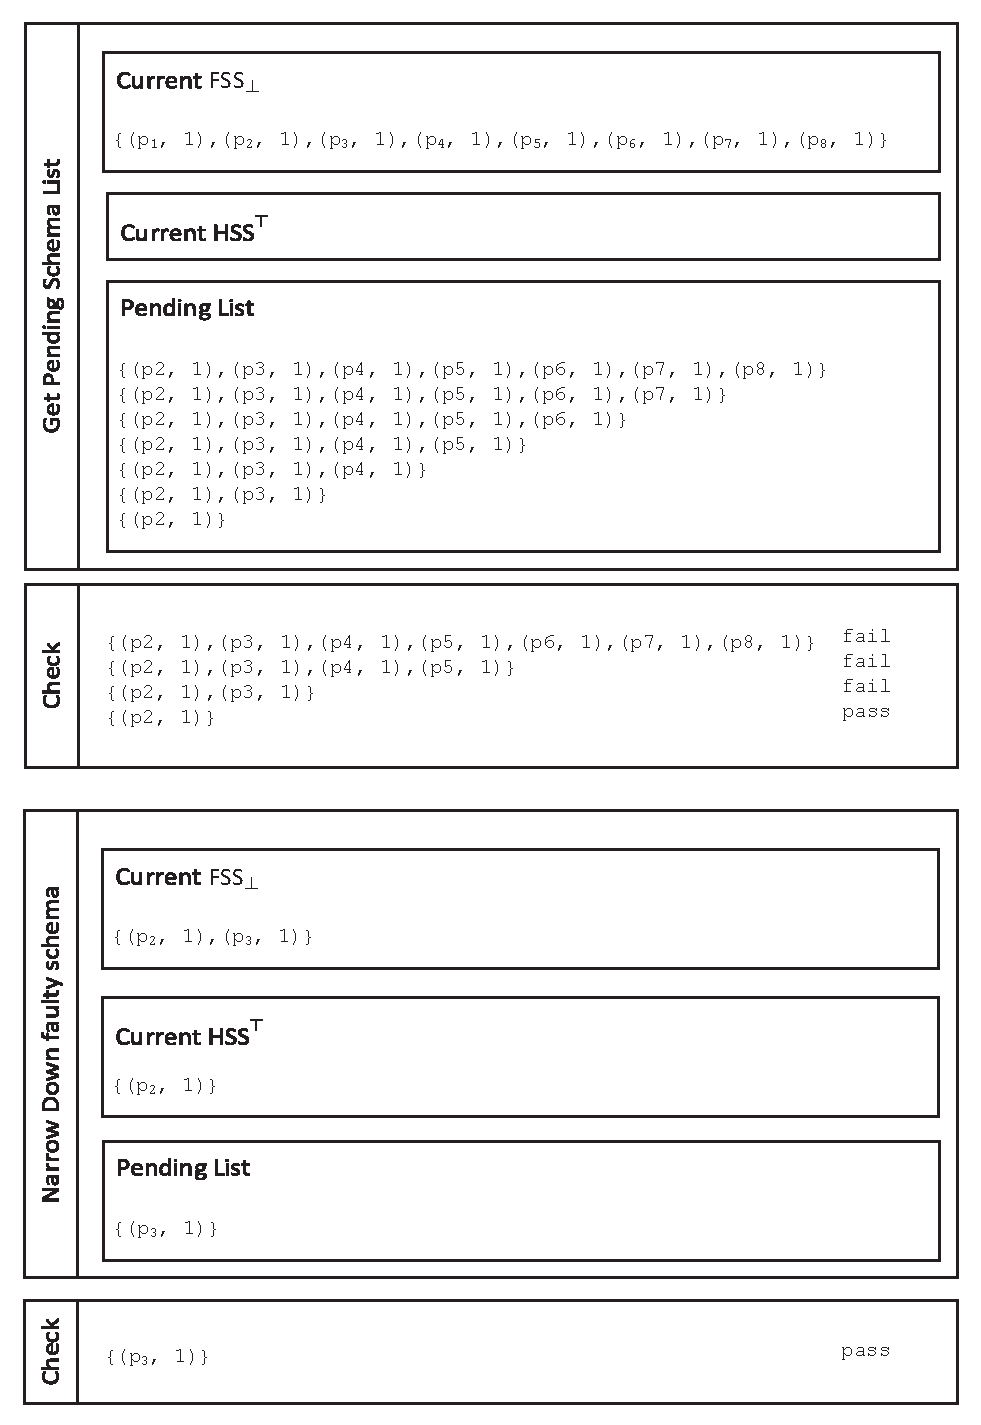
\includegraphics[width=5.8in]{exof1.eps}
 \caption{Example of Algorithm 1}
 \label{fig_exofalo}
\end{figure*}



Since we have given the algorithm to identify the MFS when given a candidate MFS, to complete the process of MFS identification, we need to know how to find these candidate MFS. Algorithm 2 describes how we can find these candidate MFS, as well as the complete process of how to identify the MFS when given a failing test case.




The input of this algorithm is a failing test case $t$, and the output is the MFS in this test case. Variable $HSS^{\top}$ records the current maximal healthy faulty schema set, and is initially assigned to be empty (line 1).   Variable $FSS^{\bot}$ records the current minimal faulty schema set, and initially have one schema, i.e., test case $t$. The first candidate MFS $fs$ is test case $t$ itself (line 3). This is because none of its subschema is found to be faulty at the beginning.

This algorithm also consists an outer loop (line 4 - 29). In this loop, we first obtain the candidate maximal pending schema set $Cxs$ (line 5) and the candidate minimal pending schema set $Cns$ (line 6). If there is no candidate MFS in the current iteration (line 7), we need to obtain one (line 8 - 22).  If we cannot obtain such candidate MFS (line 23), which indicates that all the schemas in this test case are classified into healthy or faulty, we will break the outer loop (line 24), and return the identified MFS (line 30). Otherwise, we will start the Algorithm 1 to identify the MFS (line 26), and set the candidate MFS to be Null (line 27), so that the outer loop can continue.

With respect to obtaining candidate MFS (line 8 - 22), we will first obtain a set of schemas -- $list$, which satisfies $list = $\{$c_{1}$, $c_{2}$, $c_{3}$, ..., $c_{m}$\}, where $c_{i} \prec c_{i+1}, c_{1} \in Cns, c_{m} \in Cxs$. Similar to Algorithm 1, we also select the list which has the maximal number of schemas. Note that each schema in this set is pending schema according to Formula \ref{eq:pssthird}. If we cannot obtain such set of schemas (line 10), which indicates that none schema is pending schema in this failing test case, we will return none candidate MFS (line 11) and break the loop (line 12). Otherwise, we will execute the first schema in this set (line 14 - 15). If the result shows that this schema is a faulty schema (line 15), then this schema is a candidate MFS (line 16). This is because this schema itself is a faulty schema, and all its subschemas are pending schemas. We will then break the loop (line 17) and let Algorithm 1 identify the MFS for this candidate MFS (line 26). If this schema is checked to be a healthy schema (line 18), which indicates we cannot obtain the candidate MFS in this iteration, we will update the current maximal healthy faulty schema set $HSS^{\top}$ (line 19), and then repeat the candidate MFS searching process.


\begin{figure*}
 \centering
 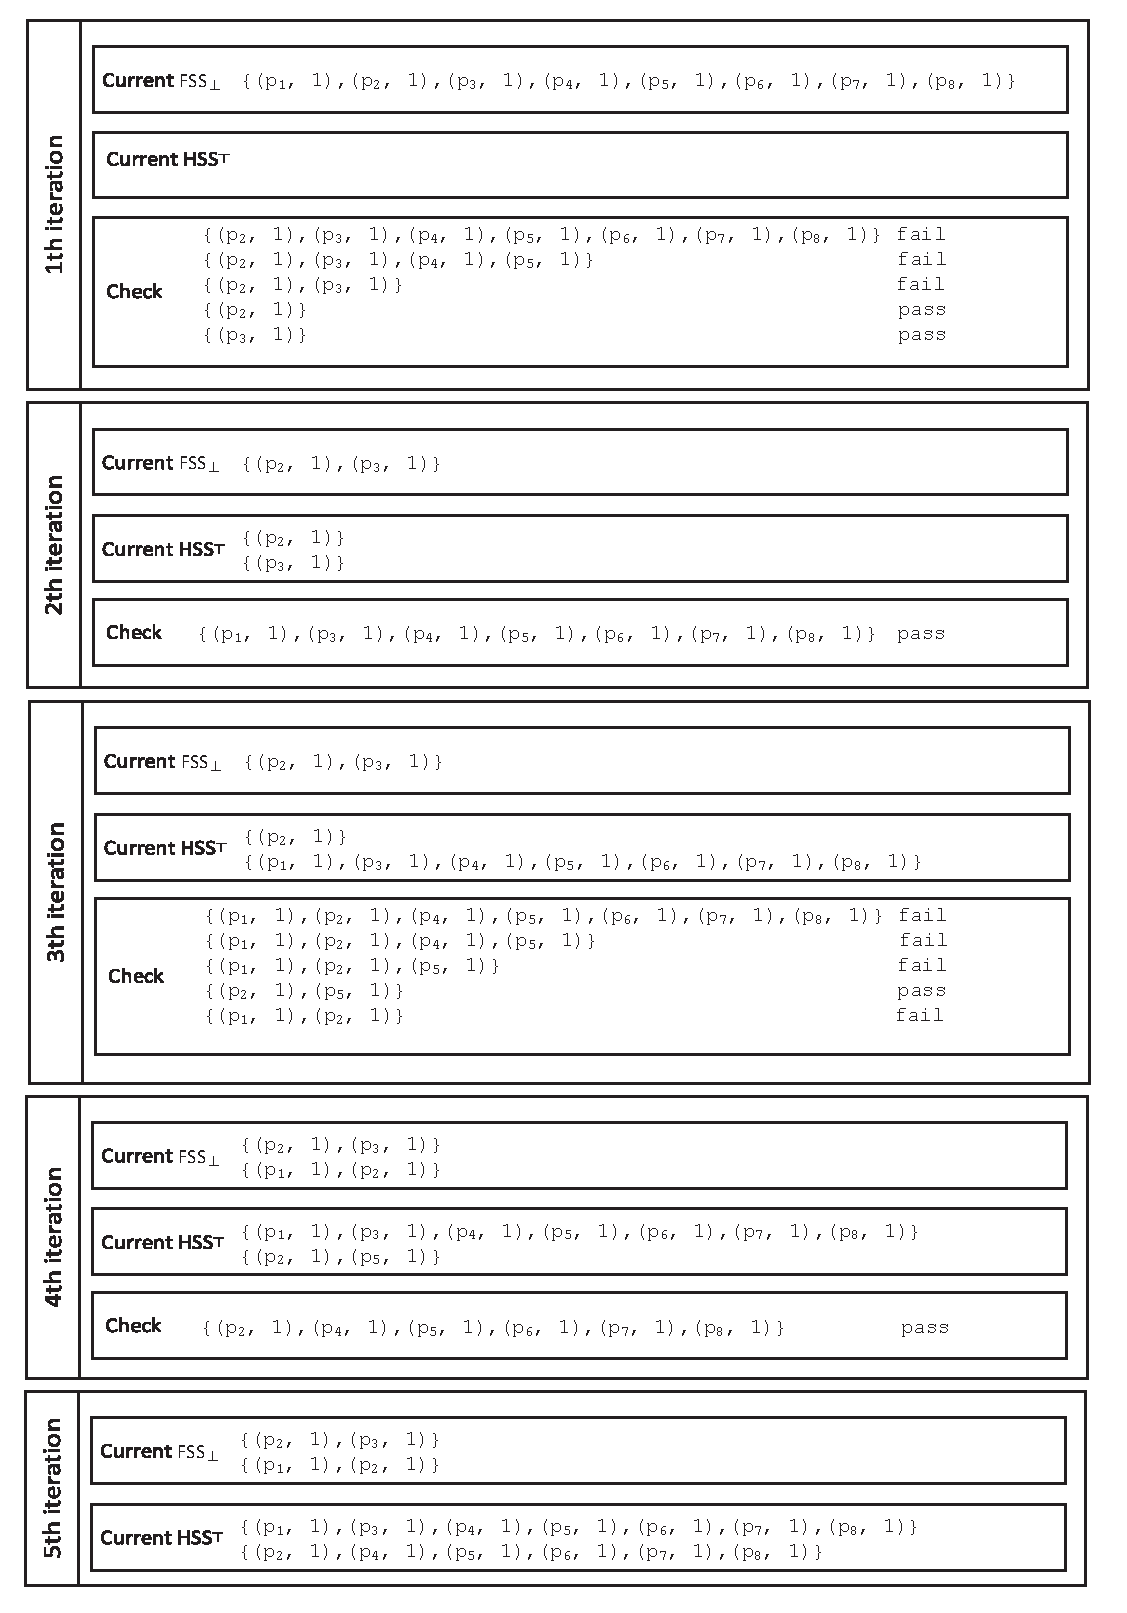
\includegraphics[width=6.1in]{exofalo2.eps}
 \caption{Example of Algorithm 2}
 \label{fig_exofalo2}
\end{figure*}



%If this list is empty, then it indicates that there is no pending schema in this test case, indicates that we have labeled all the scehams to be either, means all thes MFS is identifid in FSS.  Otherwise, we just get the fisrt one . If it fails, then its is the candaite MFS. We just need to call the algorithm to identifu thje MFS


%The overall procedure of our MFS identification approach is given as Algorithm 1.
%
%In this algorithm, $HSS^{\top}$ is the maximal set of healthy schemas, and is initially set to be empty (line 1). $FSS^{\bot}$ is the minimal set of faulty schemas, and is initially assigned to have test case $t$ (line 2). In the loop (line 3 - 14), we firstly obtaining one pending schema (line 4 - 6).  Note that $s_{p}$ must satisfy Formula \ref{eq:pssthird}, i.e., $s_{p} \in$ PSS = \{$ c\ |\ \exists c_{1}' \in Cfs$, $c \preceq c_{1}'$ $\&\&$ $\exists c_{1}' \in Chs$, $c_{1}' \preceq c$\}. In the implementation of our algorithm, we do not need to obtain all the pending schemas; instead, we just need to get one schema that is in this set. If no schema can be obtained (line 7) (indicating that there is no un-determined schema), we will break the loop (line 8), and output the MFS (line 15). Otherwise, we will check this schema to be faulty or healthy (line 10), and then update $FSS^{\bot}$ and $HSS^{\top}$ (line 11).
%
%It is noted that, in Algorithm 1, we do not describe which pending schema $s_{p}$ is obtained from the pending schemas set PSS.  How to select a pending schema is important, as it will significantly influence the speed of convergence of this algorithm, as well as the number of pending schemas we need to check to get the MFS. In this paper, we use binary search strategy to select a pending schema. Formally, let $c_{1} \in CMXS(FSS, t)$ and $c_{2} \in CMNS(HSS, t)$, $c_{1} \preceq c_{2}$. Then according to proposition \ref{pro:pending}, $\forall c_{3}, c_{1} \prec c_{3} \prec c_{2}$, $c_{3}$ is a pending schema. Without loss of generality, we can get an ordered set of pending schemas as \{ $c_{1}$, $c_{3_{1}}$, $c_{3_{2}}$, ..., $c_{3_{i}}$, ..., $c_{2}$ \}, where $c_{1} \prec c_{3_{1}} \prec c_{3_{2}}  ... c_{3_{i}}  \prec c_{2}$.  Then at each iteration, we will select the middle element in the ordered set and check it. According to Propositions \ref{pro:subofhealthy} and \ref{pro:superoffaulty}, after we determined it to be healthy or faulty, we can then determine half of schemas in this ordered set of pending schemas to be healthy or faulty. Then we will update this ordered set and repeat the binary search selecting process until all the schemas in this set are determined. Note that, to take full advantage of binary search, we need to make this ordered set as large as possible. Hence, at the first of this selection procedure, we need to select $c_{1} \in CMXS(FSS, t)$ and $c_{2} \in CMNS(HSS, t)$, such that $c_{1} \preceq c_{2}$, and $|c_{1}| - |c_{2}|$ as large as possible.



\subsection{Checking a pending schema}
In this section, we will discuss how to check a pending schema.

\begin{assumption}
Given a failing test case $t$, when we identify the MFS in $t$, any newly generated test case will not introduce new MFS that is not in $t$.
\end{assumption}

There are similar assumptions given in \cite{zhang2011characterizing,martinez2008algorithms,martinez2009locating}, and we will weaken it later. Based on this assumption, we can get the following lemma which helps to determine whether a pending schema is a healthy schema or a faulty schema.
\newtheorem{lemma}{Lemma}
\begin{lemma}
For a pending schema, we generate an extra test case that contains this schema. If the extra test case passes, then this schema is a healthy schema. If the extra test case fails, then the schema is a faulty schema.
\end{lemma}
%\begin{proof}
%According to definition of healthy schema, it is obvious that this schema is a healthy schema when the extra test case passes.
%
%When the extra case fails, this is a faulty schema (or there exists no faulty schema and this test case would not fail because the assumption says that this newly generated case will not introduce additional faulty schemas).
%\end{proof}

This lemma is easy to understand, so that we will omit the proof and just offer an example. Assume there is a failing test case \{($p_{1}$, 1), ($p_{2}$, 1), ($p_{3}$, 1), {($p_{4}$, 1), ($p_{5}$, 1)\}, and we need to check the schema \{($p_{2}$, 1), ($p_{4}$, 1)\}. According to Lemma 1, we need to generate additional test case which contains this schema, and the other parameter values in this test case should be different from the original failing test case. Based on this, test case \{($p_{1}$, 0), ($p_{2}$, 1), ($p_{3}$, 0), {($p_{4}$, 1), ($p_{5}$, 0)\} satisfies this requirement (Note that, there may exist other test cases that satisfy this requirement). If this test case fails, then \{($p_{2}$, 1), ($p_{4}$, 1)\} is a faulty schema; otherwise, it is a healthy schema.

\subsubsection{Alleviation of assumption 3}

If assumption 3 does not hold, it may lead to incorrect pending schema checking. Specifically, if the extra test case fails during testing, we cannot ensure that it is because that the pending schema is a faulty schema, or because that this extra test case contains another MFS which is not contained in the original failing test case. Consequently, we may determine a pending schema to be faulty schema while it is actually a healthy schema.

To alleviate this problem, we augment our MFS identification approach with a feedback mechanism. In detail, after we obtain the MFS with Algorithm 1, we will generate an additional distinct test case which contains the MFS, and execute it. If this test case fails, we stop the whole MFS identification procedure, and regard these schemas identified by Algorithm 1 as MFS; otherwise, we need to re-start Algorithm 1, because the MFS we identified is obviously incorrect. Note that when we re-run Algorithm 1, we can re-use some information from the test cases generated and executed at the previous iterations.

%which in high level we will validate the identify result at the end of the aforementioned algorithm, and if the schema is validated as a minimal faulty schema, we will end the algorithm, otherwise we will repeat the algorithm again to adjust the result. The detail of our augment algorithm is list in Algorithm 5.
%

%\subsection{Example}
%We will give a complete example listed in Table \ref{identifying_example}. Assume that a SUT is . constraints.
%\begin{table*}\renewcommand{\arraystretch}{1.3}
%  \caption{An example of identifying} \centering
%  \label{identifying_example}
%  \begin{tabular}{c|c|c|c|c|c}\hline
%  \hline
%  \bfseries $S_{CMINFS}$ &   \bfseries $S_{CMAXHS}$ & \bfseries Longest Chain & \bfseries Choosing Schema & \bfseries Generating Test case & \bfseries Execution result\\
%  \hline
%  1 & 1 & 1 & 1 & 1 & false \\
%   1 & 1 & 1 & 1 & 1 & pass\\
%  1 & 1 & 1 & 1 & 1 & false\\
%  \hline
%  \end{tabular}
%
%\end{table*}

\subsection{The number of additional  test cases}
There are two parts in our approach that need to generate additional test cases. First, when given a candidate MFS, it needs to generate additional test cases to get the real MFS. Second, it needs additional test cases to find the candidate MFS.

For the first part, when given a candidate MFS, according to Algorithm 1, we need to get repeats obtain a list of its pending subschemas and use binary search to check the schemas in this list. If this list happens to contain the real MFS, we only no more than $log_{2}(m)$ test cases to catch this real MFS, where $m$ is the number of parameter values in the candidate MFS. After we catch this real MFS, we still need $d\times log_{2}d$ number of test cases to check whether its subschemas are healthy schemas, where $d$ is the number of parameter values in the real MFS.


%This is because in we need to genrate maxmail list, which is equal to t. and for each list, we use binary search, so we need to log2t to get the maximal list. For each
%By the way, through to obtain this MFS, are still need to $log_{2}n$


\section{Weaken assumptions 1 and 2}
In this section we will discuss the impacts on MFS identification of the two assumptions proposed in Section \ref{sec:back}, as well as how to weaken them.

The first assumption is that the outcomes of all the tests are deterministic. In practice, re-executing the same test case may result in different outcomes. For example, if the program using some random variables, different runs of the test case will assign different
values to these random variables. Non-deterministic results will complicate the MFS identification, and even worse, it may lead to an unreliable result of the MFS identification. Inspired by the idea that using multiple same-way covering arrays to identify the MFS \cite{fouche2009incremental,yilmaz2006covering}, one potential solution to alleviate this non-deterministic failure is by adding redundancy, i.e., through re-executing the same test case to obtain the relatively stable outcome.

The second assumption is that if a test case contains a MFS, it must fail as expected. Some effects \cite{Masri:2014:PCC:2582050.2559932,yilmaz2013reducing} may make this assumption invalid. According to the study \cite{zhang2011characterizing}, we can learn that the schemas that are identified under this condition may be the super-schema of actual MFS. Hence, in practice, we may not only need to check the schemas that are identified as MFS, but also need to pay attention to their sub-schemas.

\section{Evaluation with simulated SUT} \label{sec:simulateEx}
In this section, we designed a simulated SUT of which the number of parameters and the value of each parameter can both be customized. In addition, we can also manually inject faulty schemas in the simulated SUT. We will conduct a series of experiments with this simulated SUT. The goal of our experiments is to evaluate the efficiency and effectiveness of our approach when compared with other existing techniques. The main reason that we use simulated program is that we can easily run a set of experiments with various states of a SUT, i.e., different parameters and different MFSs. By doing so we can thoroughly learn the performance of each algorithm without biases.
%In addition, we will conduct the empirical studies on some real software subjects at Section \ref{sec:realEx}.

%As we discussed in the background section, the fault privilege properties just effect the way we determine a configuration is fail or pass. It doesn't effect the performance of each algorithm. So to be simple and clear, we omit the fault privilege in the simulated SUT , i.e., all the fault in the SUT has the same privilege. This is a ideal scenario which may not exist in real softwares, in the empirical studies of section 7 we will deal with the real faults in some open-source softwares with different privileges.
\subsection{Approaches for comparison}
There are several approaches that aim at identifying the MFS, which can be classified as non-adaptive methods and adaptive methods. The former ones do not need additional test cases while the latter do. Our algorithm belongs to the adaptive methods. To make the comparison clear and fair, we select all the adaptive MFS identification in this study, which are listed as follows:

(1) OFOT \cite{nie2011minimal} -- It changes one factor of a test case one time to generate a new test case and then analyse the MFSs according to the executed result of these test cases. (2) FIC\_BS \cite{zhang2011characterizing} -- It uses a delta debugging strategy to isolate the MFSs (3) LG \cite{martinez2008algorithms,martinez2009locating} -- It uses a locatable graph to represent the faulty schema and adopts the divide and conquer strategy to find the MFSs. (4) SP\cite{ghandehari2012identifying} -- It generates test cases for the most suspicious schemas and gives a rank of these schemas. (5) CTA\cite{shakya2012isolating}, it combines the OFOT approach and the classified tree technique which is firstly applied in research \cite{yilmaz2006covering}  to analyse the MFSs. (6) RI \cite{li2012improved} -- It also uses delta debugging, but mutates a different factors  when compared with FIC\_BS. (7) AIFL \cite{wang2010adaptive} -- It extends OFOT, which changes different number of factors instead of one at each iteration for a test case. (8) TRT \cite{niu2013identifying} and (9) TRTNA \cite{niu2013identifying} --  They use a structured tree model to analyse the MFSs in a failing test case.  More details of these algorithms will be discussed in the related works. (10) Furthermore, our approach in this comparison will be denoted as CMS, which represents Candidate Minimal$\//$Maximal pending Schemas.

With respect to \emph{SP}, the degree of MFS set for this algorithm is 2 (except for the last group of experiment, which is 4 instead). We list a overview of these approaches in Table \ref{comparison-metrics}. In this table, Column ``Tests'' lists the number of additional test cases generated by each approach. These number vary from different approaches, and are related to the number of parameters, i.e., $n$, in the SUT, the number of MFS, i.e., $k$, to be identified, and the degree of MFS, i.e., $d$. Column ``Degree'' shows the degree of MFS that each approach can identify. We can learn that almost all the approaches can identify the MFS with degree ranges from 1 to $n$, except approach ``LG'', which can only identify the MFS with degree 2, and approach SP, which can only identify the MFS with degree no more than a given number $t$.  Column ``Multiple'' indicates that whether the approach can handle the condition that a failing test case contain multiple MFS. Result ``Multiple'' shows that the corresponding approach can handle such condition, while ``Single'' indicates that the approach cannot handle this type of test case. Note that some approaches can only handle the condition that multiple MFS have no overlapped part (has no same parameter value). These approaches will be labeled with ``none overlapped''.
At last, Column ``MFS introduce'' shows whether the approach can deal with the newly introduced MFS in the additional generated test cases. Signal $\oslash$ means that the corresponding approach cannot handle such case, while $\odot$ indicates that the approach is able to deal with it.

\begin{table*}[!htb]
  \caption{The overview of each algorithm} \centering
  \label{comparison-metrics}
  \begin{tabular}{c|c|c|c|c}\hline
  \bfseries Approaches & \bfseries Tests & \bfseries Degree & \bfseries Multiple & \bfseries MFS introduce \\

  \hline
    OFOT & n  & 1$\sim$n & single & $\oslash$ \\
    FIC\_BS & $k \times (d \times (log_{2}(n) + 1))$ & 1$\sim$n & multiple, none overlapped  & $\oslash$ \\
    LG & $k \times log_{2}(n) + k^{2}$  & 2 &  multiple & $\oslash$ \\
    SP & $\geq$ n  & $\leq$ d & multiple & $\odot$\\
    CTA & n  & 1$\sim$n  & single & $\oslash$  \\
    RI & $\geq$ $ k \times (d \times (log_{2}(n) + 1))$  & 1$\sim$n &  multiple, none overlapped  & $\oslash$  \\
    AIFL & $\leq$ $2^{n}$  & 1$\sim$n & multiple, none overlapped  & $\oslash$  \\
    TRT & -  & 1$\sim$n & multiple & $\oslash$  \\
    TRTNA   & - & 1$\sim$n & multiple & $\odot$  \\

      \hline
    CMS & O(log(n)) & 1$\sim$n & multiple   &  $\odot$ \\

  \hline
  \end{tabular}

\end{table*}


\subsection{Evaluation metrics}
There are two focuses in this study: 1)How many additional test cases do these approaches need to generate? 2) The effectiveness of these approaches?  We apply recall and precision to evaluate the second question :
$$recall =
 \frac{correctly\ Identified\ MFS}{all\ the\ MFS\ in\ SUT}
$$

$$precision =
 \frac{correctly\ Identified\ MFS}{all\ the\ identified\ MFS}
$$

\emph{Recall} measures how well the real MFS are detected and identified. $Precision$ shows the degree of accuracy of the identified schemas when comparing to the real MFS.

%The recall is percentage of the correctly identified MFSs of an algorithm of all the MFSs in the SUT. The bigger the metric the better an approach can perform on finding MFSs in a SUT. There are some factors may influence this metric of an algorithm, mainly are whether an approach consider a failing configurations contain multiple MFSs, whether consider if there exist overlapped MFSs in a failing configurations and whether consider the newly introduced MFSs of the additional generate configurations.  The precise is the percentage of the number of correctly identified MFSs of algorithm of all the number of  MFSs this algorithm identified. This metric measure the accurately of an approach and the bigger it is the better the approach performs. This metric is related to whether a algorithm consider the influence if an generated test case contain newly MFSs. If the approach did not consider so, it may make a wrong judgement to determine some schemas in the original configuration to be faulty schemas which in fact are not.
%
%Of course these factors we mentioned are just affect these the no-machine learning algorithm, as for the machine learning algorithms,i.e., CTA, the factor that matters is the classified algorithms itself.


\subsection{Experiment setups}
We will carry out the following five experiments in this section:

1)For the first one, we will give a set of SUTs with 8 parameters, each parameter has 3 values ($3^8$). We inject each of them with only one distinct 2-degree MFS. There are $\binom{8}{2} = 28$ possible MFSs we can inject for a test case with 8 parameters, hence, the number of SUTs in this study is 28. For each SUT in this set, we will feed each approach a failing test case with the MFS contained in it, and then let these approaches identify the MFS. We will record the additional test cases each approach needed, as well as the precision and recall with respect to the identified MFS.

% This experiment will give us a initial view of the cost of each algorithm on identifying the MFS in a failing test case.

2)The second experiment is similar to the first one, except that we will inject two different 2-degree MFSs in each SUT. It is easily compute that there are $\binom{28}{2} = 278$  possible SUTs in this experiment. We also feed these approaches with a failing test case that contains the injected two MFSs and then let them identify the MFS.
%Another difference from the experiment 1 is that in this experiment we will record the "recall" and "precise" of each algorithm, as these metric is not equal to 1 for all the algorithms like experiment 1. This experiment mainly focus on observing the performance of each algorithms in facing multiple MFSs in a configuration.

3)The third experiment aims at measuring capability of each algorithm at handling the  newly introduced MFSs. To accomplish this goal, We firstly inject two MFSs in a SUT, and then feed each approach a failing test case which contains only one 2-degree MFS, with another 1-degree MFS not in it (Note that 1-degree MFS can be easily introduced by just changing one factor of the original failing test case). There are $\binom{8}{2} \times \binom{8}{1} = 224$ possible SUTs in this experiment.


4)For the fourth experiment, we will take 8, 9, 10, 12, 15, 20, 30, 40, 60, 80, 100, and 120, respectively,  as the number of parameters of SUT. For each number of parameters, say \emph{n}, we will generate $\binom{n}{2}$ SUTs, each of which will be injected a single distinct 2-degree MFS. For these SUT, we will follow the same process as experiment 1. We will record the average number of additional test cases that each approach needed for each number of parameters. The goal of this experiment is to determine the influence of the number of parameters of SUT on each approach.

5)In the fifth experiment we will fix the number of parameters of SUT to be 8, but vary the number of degrees of the MFS that we inject in the SUT. That is, we will inject the MFS in SUT with degrees 1, 2, 3, 4, 5, 6, 7, and 8, respectively. For a degree of \emph{m} (\emph{m} = 1, 2, 3, 4, 5, 6, 7, and 8), we will generate $\binom{8}{m}$ SUTs with different m-degree MFS injected. Then we will let all those approaches identify the MFS in them. This experiment helps to inspect whether these approaches can handle different degrees of MFS in a failing test case.

\subsection{Result and discussion}
%We will discuss the results into five groups according to the experiment setups.

1)The results of the experiment 1 are depicted in figure \ref{fig_single}. The y-axis represents the number of test cases and the x-axis represents SUT with different MFS injected. The polygonal lines represent the results for each corresponding approach.
For a particular approach, a point in its polygonal line indicates the number of test cases (y-axis) needed for identifying the MFS in the SUT (x-axis).

There are some observations we can learn from this figure. First, the test cases that are needed of some approaches did not change along with the MFS we injected. These approaches are AIFL, SP, CTA, OFOT, and LG, respectively, while others need different test cases according to the MFS that they need to identify. Second, some approaches (AIFL, SP, TRTNA, OFOT, CTA) showed an obvious disadvantage, they need much more test cases than the remaining approaches. For the remaining approaches, the disparity of their results is not significant. From a deeper insight of this figure, we can conclude an initial rank in the number of test cases each approach needed as:  $FIC\_BS < RI < LG < TRT < CMS < OFOT = CTA < TRTNA < AIFL < SP$.

\begin{figure}
 \centering
 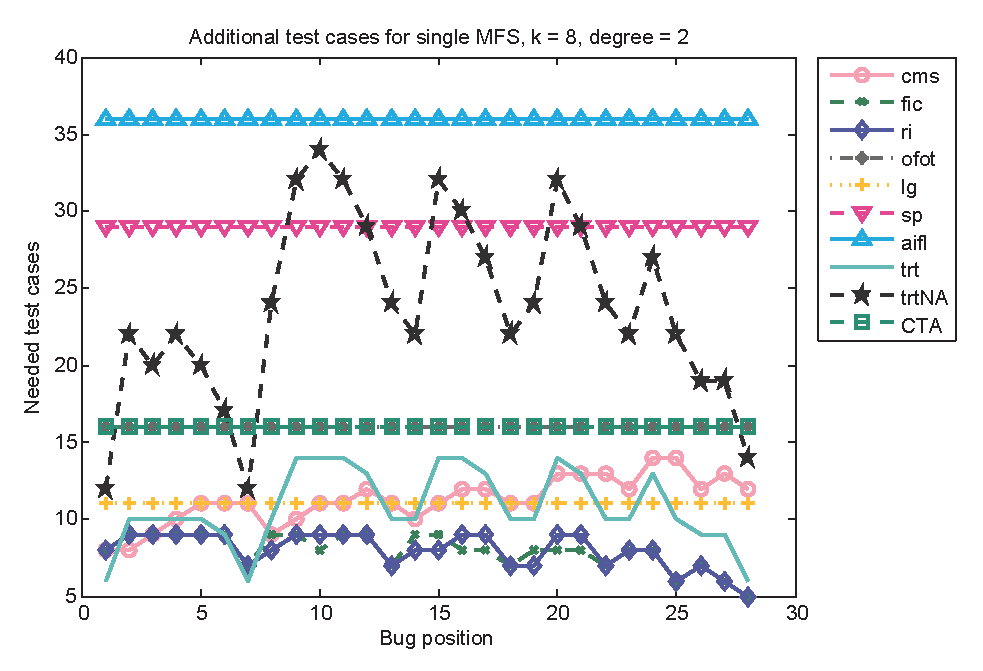
\includegraphics[width=3.4in]{single.eps}
 \caption{k = 8, t = 2,single, additional test suites}
 \label{fig_single}
\end{figure}

With respect to the precision and recall, all these approaches obtain the same performance (both precision and recall are 1). This is because the SUT with single 2-degree MFS is a very simple scenario, at which all these approaches can identify the MFS.

%From the first study, we can find that although our approach is not the best at cost, but it beat most, and not bad more than those best.

2)Figure \ref{fig_double} gives the results of experiment 2. This figure does not show the number of test cases of each approach generated, instead it just shows the average precision and recall for each approach as not all the approaches can both get recall of 1 and precision of 1 as experiment 1. It is obvious meaningless if we compare two approaches, when one of them can obtain recall of 1 and precision of 1 while the other can not.
%So we will only list the average number test cases of these approaches that can reach recall 1 and precise 1 later.

From Figure \ref{fig_double}, we can find the following approaches: CMS, LG, SP, AIFL, TRT and TRTNA can obtain 1 for both precision and recall, which means that they can properly handle the multiple MFSs in a failing test case. In the opposite case, approaches OFOT and CTA get 0 for both recall and precision. This result shows that these two approaches can't handle multiple MFSs in one failing test case. As for the remaining approaches RI and FIC\_BS, they obtained precision of 1, but did not obtain recall of 1. This is because they can't handle the condition when two MFSs have overlapped part. Under that condition, they can identify only one MFS.

%The average number of test cases of these approaches can both get recall and precise 1 is as follows:
%
%we can find that our approach can also get a no-bad result among them.

\begin{figure}
 \centering
 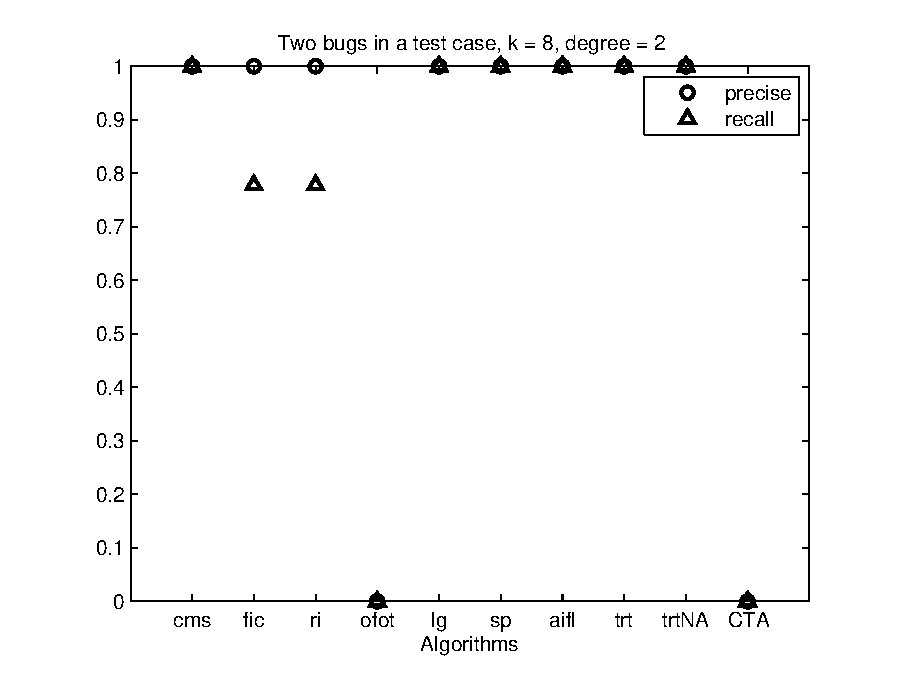
\includegraphics[width=3.4in]{d-8-2.eps}
 \caption{k = 8, t = 2,double, additional test suites}
 \label{fig_double}
\end{figure}

3)The results of the third experiment are shown in fig \ref{fig_import}. Similar to experiment 2, this figure just records the recall and precision of each approach. There are several observations in this figure.

First, no approach can obtain 1 for both recall and precision in this experiment, which indicates that no approach can fully resolve the new MFS introducing problem.

Second, there are some approaches, i.e., OFOT, LG, SP, TRTNA, and our approach CMS, that can obtain precision of 1. It indicates that the newly introduced MFS has little impact on the accuracy of MFS they identified.

Third, our approach CMS get the highest score at recall, and the specific rank are $CMS > OFOT > LG = SP = TRTNA > CTA > AIFL > TRT > FIC\_BS = RI$. It shows that our approach can find more MFSs than others when just given a failing test case.

Fourth, approaches FIC\_BS and RI really suffer from the new MFS introducing problem, because they get 0 at both recall and precision.

\begin{figure}
 \centering
 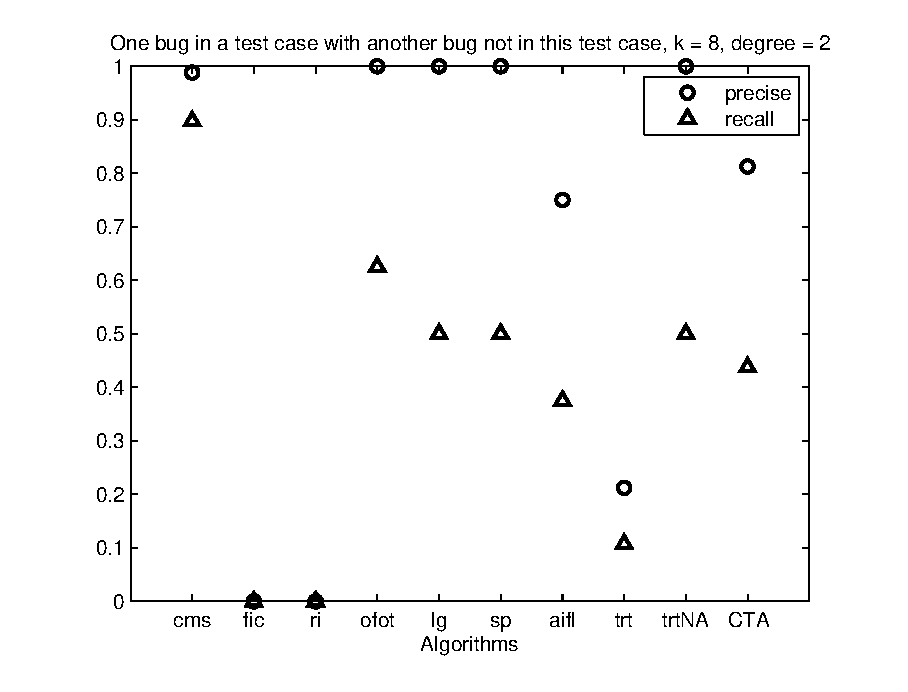
\includegraphics[width=3.4in]{i-8-2.eps}
 \caption{k = 8, t = 2,import, additional test suites}
 \label{fig_import}
\end{figure}

4)Figure \ref{fig_free_k} depicts that the average test cases needed of each approach for experiment 4. In this figure, the y-axis represents the number of test cases, and the x-axis represents the number of parameters of the SUT. The number of parameters are 8, 9, 10, 12, 15, 20, 30, 40, 60, 80, 100, and 120, respectively.  A point in this figure indicates the average number of test cases needed to identify the MFS in the SUT with the corresponding number of the parameters. Note that in this figure, the average numbers of test cases of approaches SP, AIFL, OFOT and CTA increase quickly with the increase of k. It could make the results of the remaining approaches unclear if we put all of them in the same figure. Hence, we just show the results of the remaining approaches (TRTNA, TRT, LG, CMS , FIC\_BS, and RI), and offer a smaller figure  which shows the results of all the approaches.

We can easily learn that AIFL needs the largest number of test cases to identify MFS. Even worse, the computing resource that it needs also increases quickly along with the increase of k. Consequently we cannot use this approach to identify the MFS in the SUT with number of parameters larger than 12. Approach SP performs the second worst in this experiment. In fact, we cannot record its results when the number of parameters is greater than 40. OFOT and CTA are the third worst approaches in this experiment, with the number of test cases increases linearly with the increase of k.

\begin{figure}
 \centering
 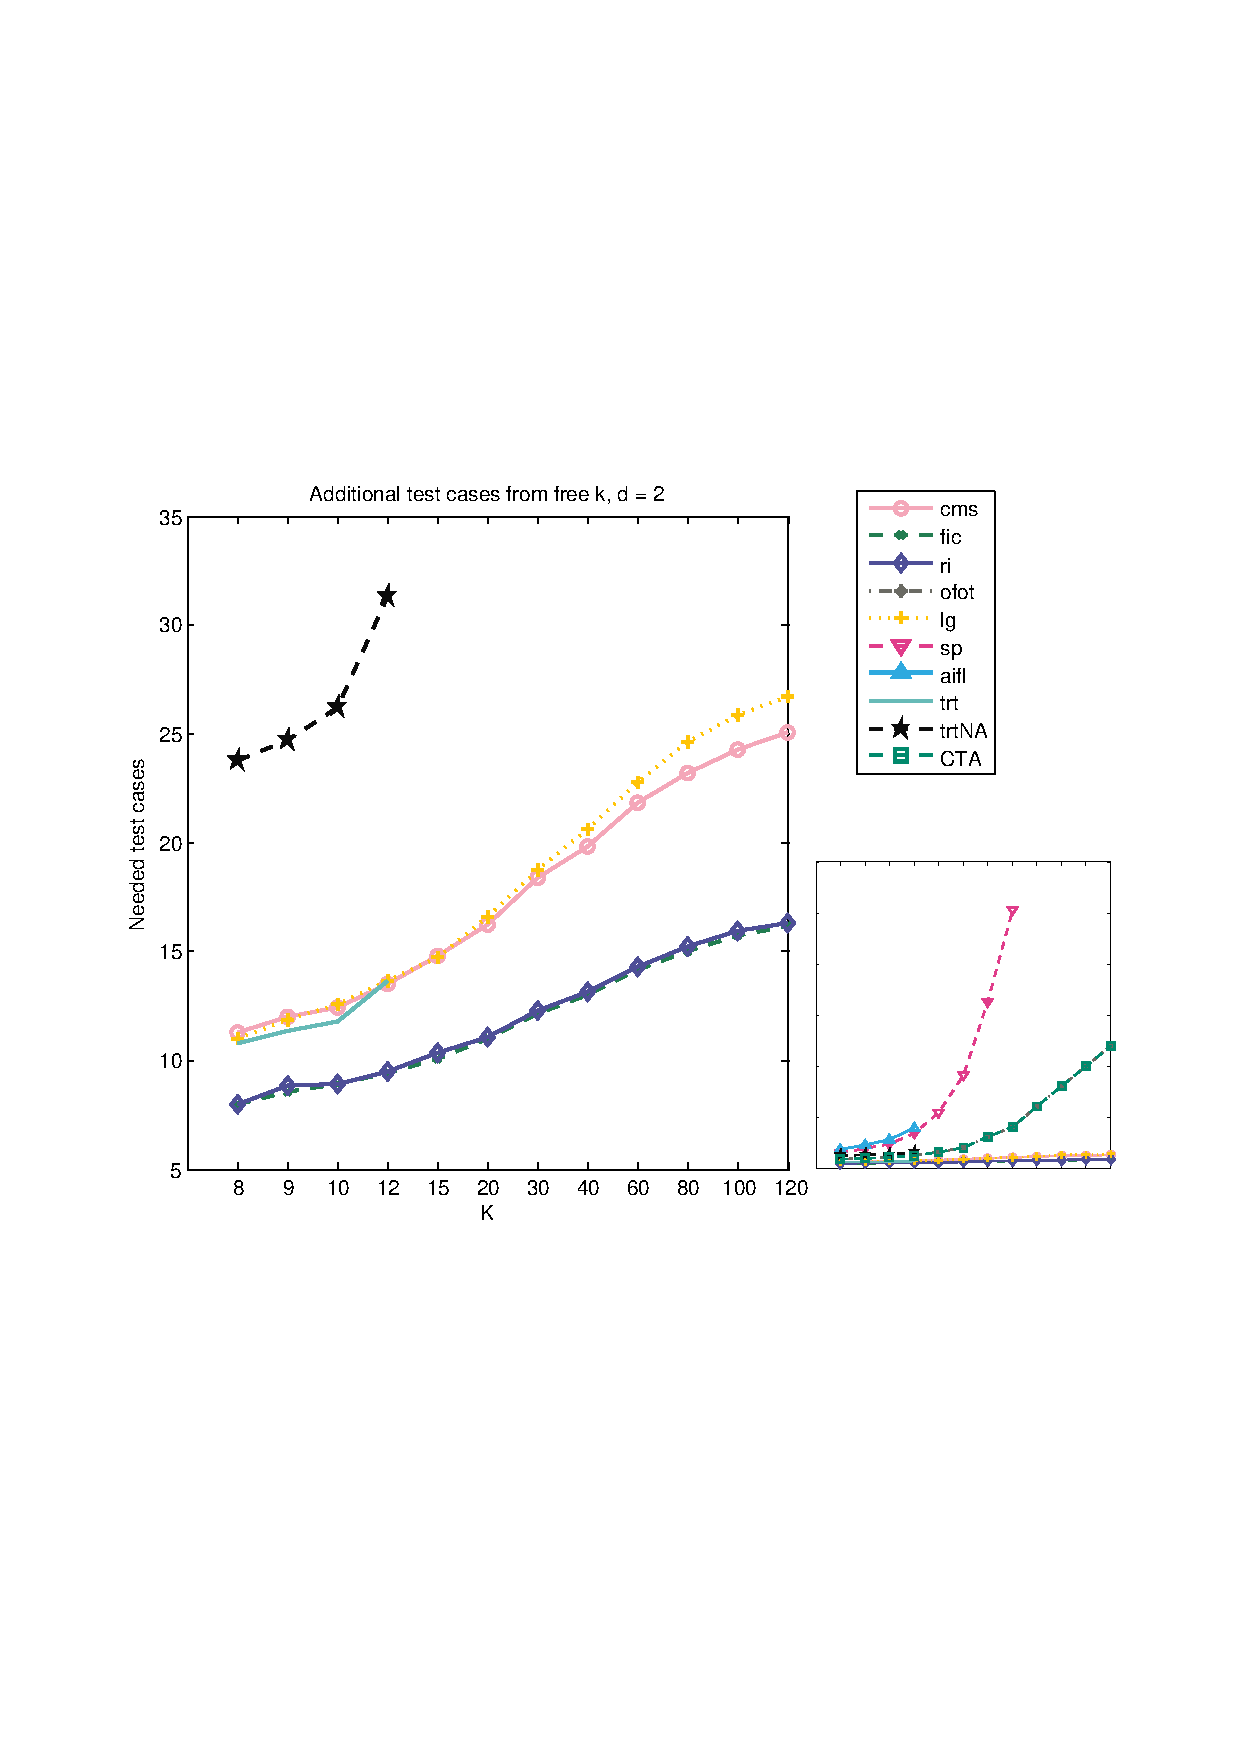
\includegraphics[width=3.4in]{cpp.pdf}
 \caption{k is free, t = 2,single, additional test suites}
 \label{fig_free_k}
\end{figure}

The remaining approaches need much smaller number of test cases than four previously discussed approaches. Among these approaches, however, TRT and TRTNA cannot identify the MFS in the SUT with k greater than 12 (Due to their high computing complexity). Apart from this two approaches, all the remaining approaches, i.e., CMS, FIC\_BS, LG, and RI can quickly identify the MFS for different values of k. We can conclude a rank of these approaches according to the number of test cases generated, $AIFL > SP > TRTNA > OFOT = CTA > LG > CMS > TRT > RI > FIC\_BS$.


5)Figure \ref{fig_free_d} depicts the results of the last experiment. This figure is organised similarly as figure \ref{fig_free_k}, except that the x-axis in this figure represents the degree of MFS we inject in it. For a particular approach, a point in this figure shows the average number of test cases needed to identify the MFS. Note that in this experiment we set the degree of MFS that SP can identify to be 4 (In this experiment, SP can only identify the MFS with degree no more than 4). As a result, the number of test cases that SP need to identify the MFS in a failing test cases increases a lot than before, which is much more than the remaining approaches. Hence, we first show the results of the remaining approaches, and offer a smaller figure which added the results of SP.

%to distinguish with algorithm LG which can just identify the MFS with degree not bigger than 2.

Some observations in this figure includes:  First, LG can only identify the MFS with degree no more than 2.  Second, we can find the numbers of test cases of RI and FIC\_BS increase quickly along with the increase of degree. Third, CTA and OFOT need the same number of test cases, i.e., 16, regardless of what the degree is. Fourth, although AIFL perform the worst in most cases, it can do better than other approaches under a high degree (7 and 8).  Fifth, the numbers of test cases needed by TRTNA, TRT and our approach CMS increase slowly with the increase of degree.

\begin{figure}
 \centering
 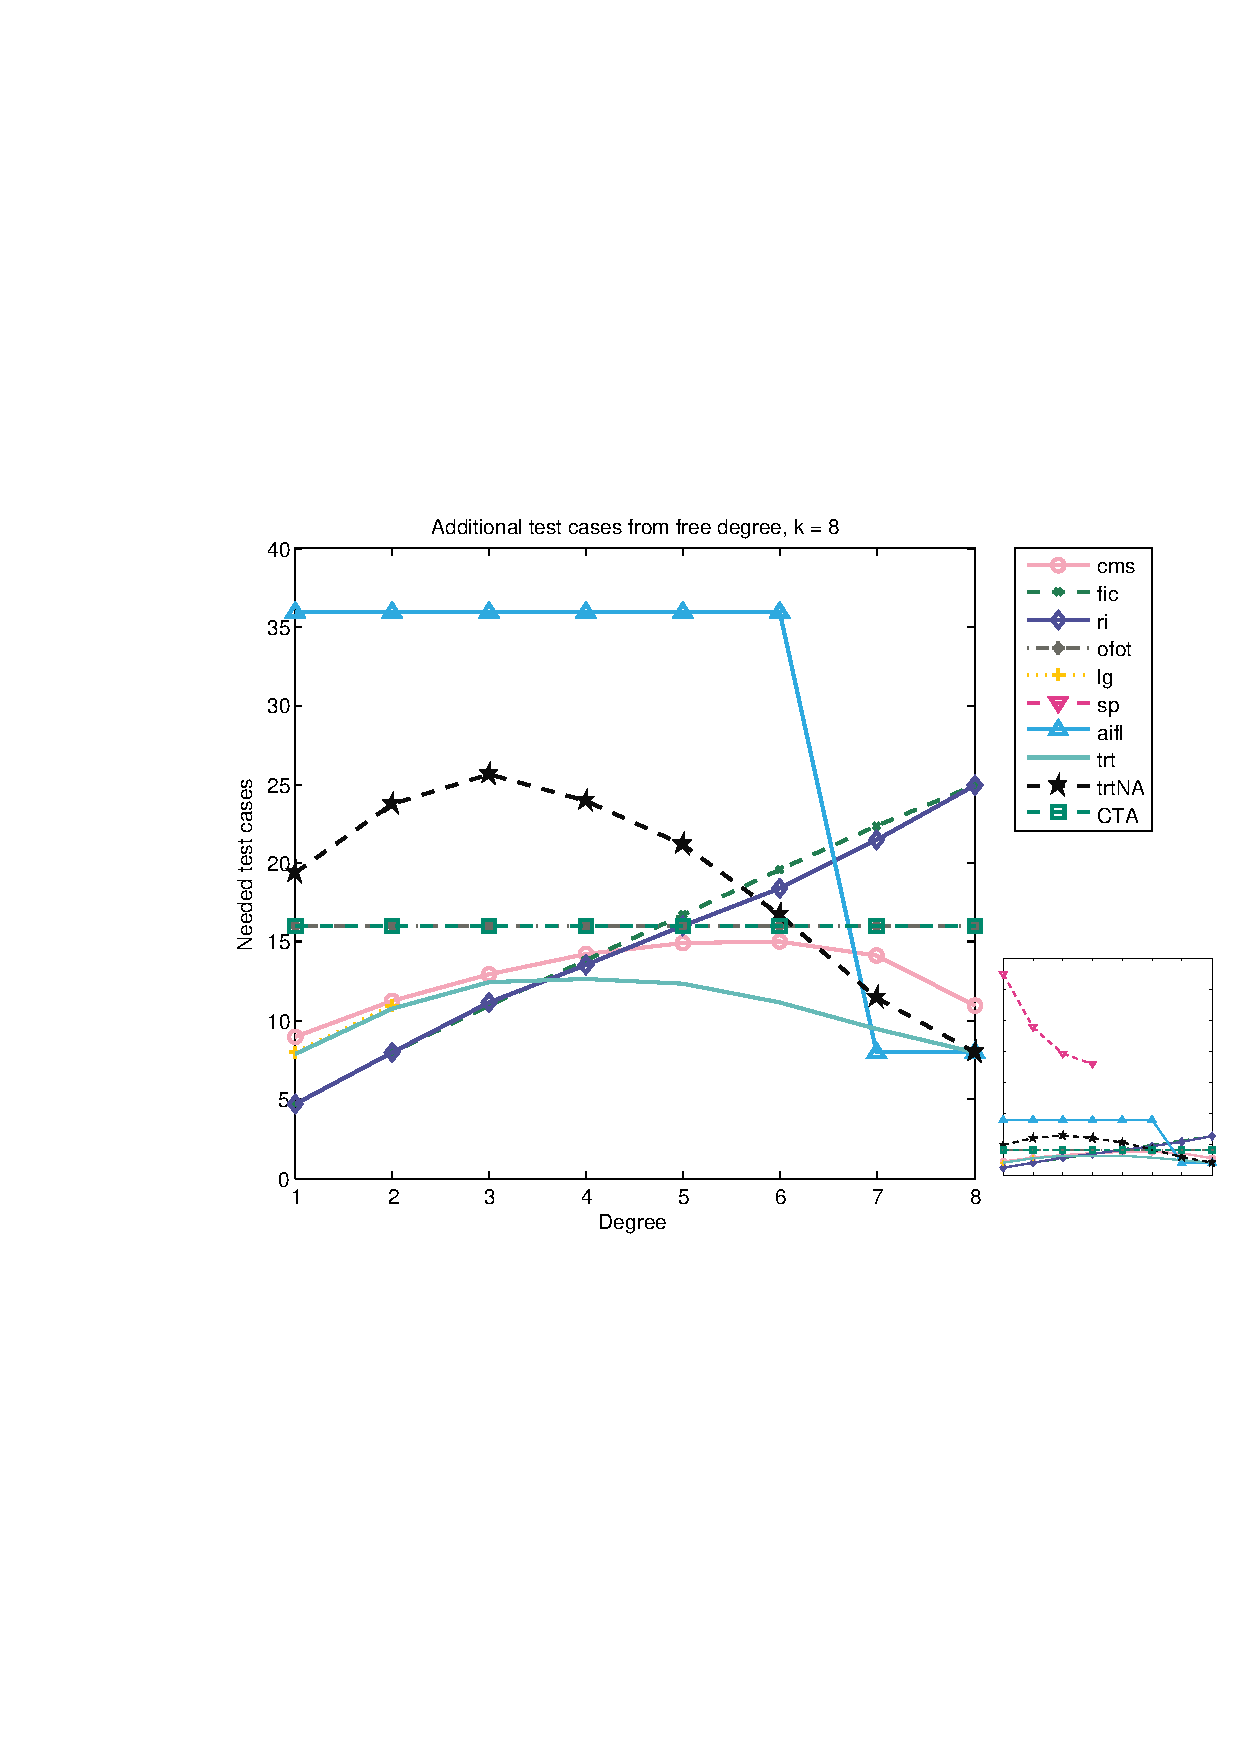
\includegraphics[width=3.4in]{cpp2.pdf}
 \caption{k = 8, t is free,single, additional test suites}
 \label{fig_free_d}
\end{figure}

In summary, our approach obtains good values at recall and precision with respect to the MFS identification, while generates much smaller number of test cases than most existing approaches. Furthermore, our approach performs better than most existing approaches under the following conditions: multiple MFS in one test case (Especially the MFS having overlapped part), new  MFS introducing problem, SUT with a large number of parameters, and MFS with a high degree.

%we will enlarge some of them to figure

\section{Empirical Case study}\label{sec:realEx}
% While we got know that our approach have a better performance than others in several scenarios such as a failing test case contains multiple MFSs, the generated extra test case introduces newly MFS and so on from previous simulated experiments, it did not give us strong confidence in that our approach will also perform well in real software systems. One important reason of this is that we don't know whether these competitive scenarios for our approach existed in real software systems. So to eliminate the doubt we conduct a series empirical studies in this section.
In this section, we will conduct the empirical study on several real-life software subjects.


% These empirical studies aimed to answer the following questions:

% Q1:Is there any test case that contain multiple MFSs, and if so, do they overlapped each other? Do any of these MFSs have high degree and how likely does it introduce newly MFS when generate extra test cases.
%
% Q2:How well of these approaches mentioned in previous sections performed when identifying the MFS in the real softwares?
%
% Q3:If we combine the result of one approach with another one, does it give us a better result than both of them?

%The subject systems for these studies are HSQLDB(2.0rc8). HSQLDB is a database management system written in pure java. All of them have millions of uncommented lines of code. And they all share the same proceedings depicted in  when tested in the following studies.


%Fig.\ref{proceeding}

%\begin{figure}
% \centering
% 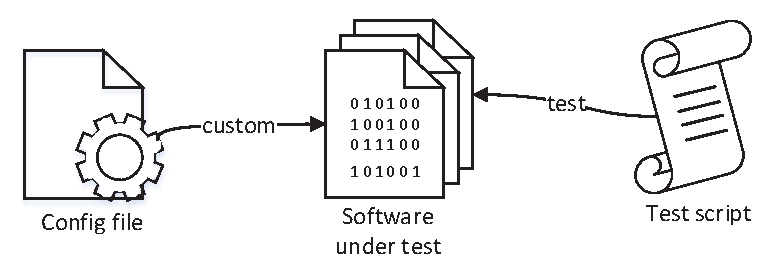
\includegraphics[width=2.7in]{proceed.eps}
% \caption{proceeding}
% \label{proceeding}
%\end{figure}

%As see from the figure, there are three modules in this proceeding: configuration file, software under test and the test script. The software under test is a set of software components which supply some interfaces, with which one can invoke the serving functions of the software. The configuration file is the file that can custom the properties of the software, and the test script is a executable file which test some functions of the software. In specific, the proceeding is trying different configuration of the software by changing the content of the configuration file, and then executing the same test script to observe the result.

%\subsection{experimental setup}
%Before we use these programs for study, we will take the following steps for each program to obtain the basic information of them, 1)Build the input configuration model of the subject program 2)execute the test case under each possible configuration and record their executed result. 3)list all the types of fault during testing and judge their priority.
%
%We will depict these processes and results for each subject program in detail.

\subsection{Subject programs}\label{sec:subject}
The subject programs used in our experiments are listed in Table \ref{subject}. Column ``Subjects" indicates the specific software. Column ``Version" indicates the specific version that is used in the following experiments. Column ``LOC" shows the number of source code lines for each software. Column ``Faults" presents the fault ID, which is used as the index to fetch the original fault description from the bug tracker for that software. Column ``Lan" shows the programming language for each software (For subjects written in more than one programming language, only the main programming language is shown).  We select these software as subjects because their behaviours are influenced by various combinations of configuration options or inputs. For example, the component \emph{connector} of Tomcat is influenced by more than 151 attributes \cite{tomcatconnector}.

\begin{table}[ht]
\caption{Subject programs}
\label{subject}
\centering
\begin{tabular}{l|l|l|l|l}
\hline
Subjects & Version & LOC & Faults &  Lan \\
\hline
Tomcat   &   7.0.40      & 296138    &   \#55905  & java  \\
Hsqldb   &   2.0rc8  &   139425   &    \#981  & Java \\
Gcc      &   4.7.2      &  2231564   & \#55459   &  c\\
Jflex    &    1.4.2     & 10040    &    \#87   & Java \\
Grep     &   2.12       & 27046   &    \#7600  & c \\
Cli      &   1.3.1      & 6433    &    \#265   & java  \\
Joda     &   2.8.2      & 85026   &    \#297   & java \\
Lang     &   3.4        & 66047  &     \#1205  & java \\
Jsoup    &    1.8.3     & 10295   &    \#688   & java \\

 \hline
\end{tabular}

\end{table}

To conduct this study, we firstly must know the faults and their corresponding MFS in prior, so that we can determine whether the schemas identified by different approaches are accurate or not. For this, we looked through the bug tracker of each software and focused on the bugs which are caused by the interaction of configuration options. Then for each such bug, we obtain its MFS by analysing the bug description report and the associated test file which can reproduce the bug.

%Among these subjects, Tomcat is a web server for java servlet; Hsqldb is a pure-java relational database engine; Gcc is a programming language compiler; Jflex is a lexical analyzer generator; and Tcas is a module of an aircraft collision avoidance system.






%To make the testing process can definitely find failing test cases (otherwise we may not detect any fault and then there is no difference between our approach with traditional approach), we prepared fault version of these software in prior. There are four software, we take the real failures, for each failure, there bug tracker can be find .  The last one is the injected failure, which is originally injected in
%\subsection{Testing buliding}.
%\subsection{Tomcat}
%
%\subsection{JFlex}
%
%\subsection{HSQLDB}
%
%\subsection{GCC}
%
%\subsection{Tcas}


\subsubsection{Specific inputs models}

To apply MFS identification approaches on the selected software, we need to firstly model their input parameters. It includes the options that cause the specific faults in Table \ref{subject}, and some additional options, which are used to create some noise for the MFS identification approach.
% Details of the specific options and their corresponding values of each software are posted at \texttt{http://gist.nju.edu.cn/doc/ict/}.
A brief overview of the input models as well as the corresponding MFS (degree) is shown in Table \ref{inputs}.

%As our study is focus on combinatorial testing,
% we must take the faults,  Some faults we collected are it. To let our CT model more applied. We add some additional options that can happen interactive events to them. We let them . To get the real MFS, note that the additional , we need to exhaustive execute all the test cases, so that we limited them at a moderate level.

\begin{table}[ht]
\caption{Inputs model }
\label{inputs}
\centering
\begin{tabular}{l|l|l}
\hline
Subjects & Inputs & MFS \\
\hline
Tomcat   &  $2^{8} \times 3^{1} \times 4^{1}$       & 1(1) 2(2)  \\
Hsqldb   &   $2^{9} \times 3^{2} \times 4^{1}$      &  3(2) \\
Gcc      &   $2^{9} \times 6^{1}$      &    3(4)  \\
Jflex    & $2^{10} \times 3^{2} \times 4^{1} $        &   2(1)   \\
Grep     &  $2^{5} \times 3^{1} \times 4^{1} $   & 2(3) \\
Cli      &  $2^{8}$   & 3(1)  \\
Joda     & $2^{5}\times 3^{2} \times 5^{1}$   & 2(1) \\
Lang     &  $2^{4}\times 3^{3}$   & 2(1) \\
Jsoup    &   $2^{8}\times 3^{1}$  & 2(6) \\
 \hline
\end{tabular}

\end{table}
In this table, Column ``inputs" depicts the input model for each version of the software, presented in the abbreviated form $\#values^{\#number\ of\ parameters} \times ...$, e.g., $2^{9} \times 3^{2} \times 4^{1}$ indicates the software has 9 parameters that can take on 2 values, 2 parameters can take on 3 values, and only one parameter that can take on 4 values. Column ``MFS" shows the degrees of each MFS and the number of MFS (in the parentheses) with that corresponding degree.

Note that these inputs just indicate the combinations of configuration options. To conduct the experiments, some other files are also needed. For example, besides the XML configuration file, we need a prepared HTML web page and a java program to control the startup of the tomcat to see whether exceptions will be triggered.
%Other subjects also need some corresponding auxiliary files (e.g., c source files for GCC, SQL commands for Hsqldb, and some text for Jflex). Additionally, there are two constraints among the subjects. The first constraint is from Tomcat, of which the error page location must not be empty. The second one is from Hsqldb, of which you can only process with the ``\emph{next()}'' method in a non-scrollable result set.


\subsection{Study setup}
For each subject program listed in Table \ref{subject}, we firstly obtain all of the failing test cases. Then, for each failing test case, we will feed it to each MFS identification approach and let them identify the MFSs. Then we will compare the schemas identified by each approach with the real-life MFSs we obtained in prior. We will record the number of generated test cases, the precision, and the recall. To be fair, no other information is given to each approach except the feeded failing test case. We will repeat this comparison for each failing test case. At last, we will give the average number of test cases, precision and recall for each approach.
%
%As we will take a large number of configurations to identify( 147472 for HSQLDB), this is too big compact to some algorithms, such as TRT, IterAIFL, they can't even accomplish the task. Some other algorithm can complete this task but with a huge time cost, such as SP, it will take weeks or even months to complete. We will omit these algorithms in our comparison to make this study available in a relative short time. As a result, we just choose ChainFeedBack , FIC, RI, OFOT, LG, CTA as our comparison algorithms.

\subsection{Results and analysis}

\begin{figure}
 \centering
 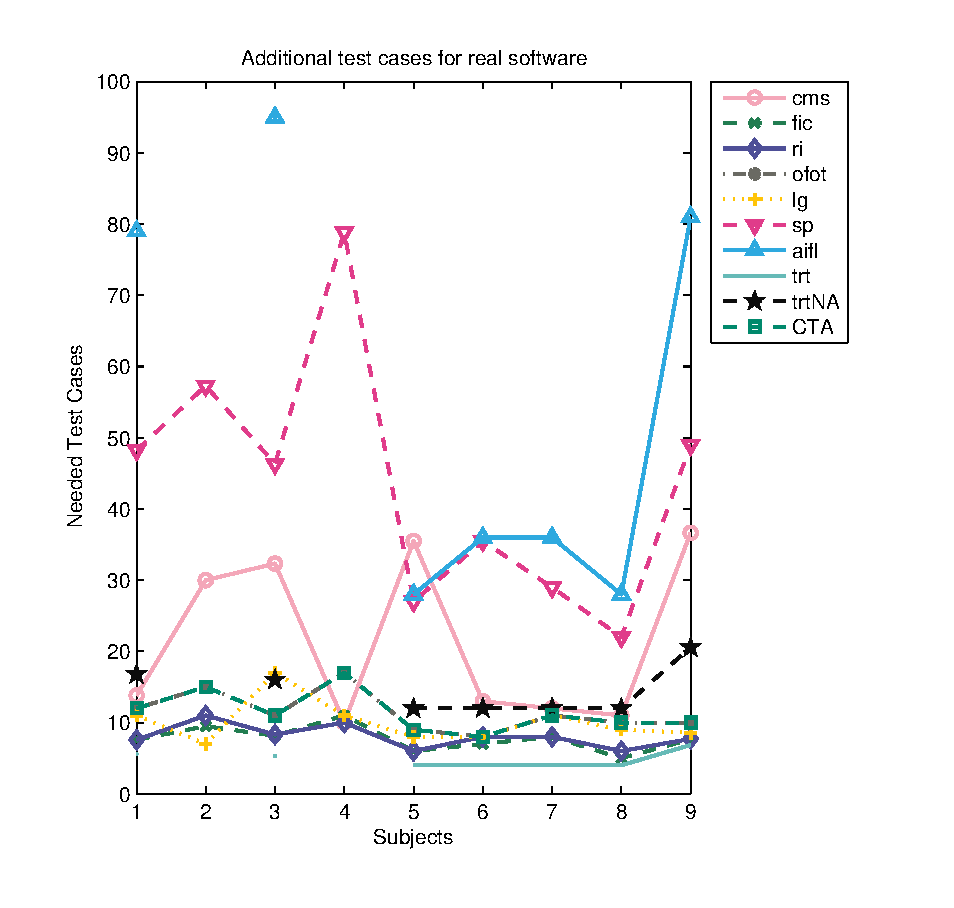
\includegraphics[width=3.4in]{num_r.eps}
 \caption{Additional test suites for real-life software subjects}
 \label{fig_realNum}
\end{figure}

Figure \ref{fig_realNum} depicts the number of generated test cases of each approach. In this figure, the y-axis represents the number of test cases, and the x-axis represents the subject programs. Each point of corresponding approach shows the average test cases generated for identifying the MFS in the SUT. It is noted that for approaches AIFL, TRT, and TRTNA, they cannot identify the MFS in subject 2 and 4 because of their large configuration space.

From this figure, we can learn that approaches AIFL, and SP generated much more test cases than the remaining approaches.  Approaches TRT, LG, FIC\_BS, needed the smallest number of test cases. The remaining approaches are in between. It is noted that our approach performed good for subjects 1, 4, 6, 7, and 8, but needed many test cases for subjects 2, 3, 5, and 9. We believe this is because for those subjects, there are too many faults (there are 2, 4, 3, and 6 MFSs for these subjects) in their test cases, which may result in many new MFS introducing problem such that our approach repeated checking the results.

% Table generated by Excel2LaTeX from sheet 'Sheet1'
\begin{table}[htbp]
  \centering
  \caption{The precision of approaches for 9 real-life software }
  \addtolength{\tabcolsep}{-1pt}
    \begin{tabular}{c|c|c|c|c|c|c|c|c|c} \hline
    App   & \multicolumn{9}{c}{Precision} \\ \hline
    CMS   & 0.7   & \textbf{1} & 0.58  & \textbf{1} & \textbf{1} & \textbf{1} & \textbf{1} & \textbf{1} & 0.27 \\
    FIC\_BS & 0.7   & 0.5   & 0.17  & \textbf{1} & 0.33  & \textbf{1} & \textbf{1} & \textbf{1} & 0.07 \\
    RI    & 0.7   & 0.5   & 0.17  & \textbf{1} & 0.33  & \textbf{1} & \textbf{1} & \textbf{1} & 0.07 \\
    OFOT  & 0.8   & \textbf{1} & 0.67  & \textbf{1} & 0.39  & \textbf{1} & \textbf{1} & \textbf{1} & 0.43 \\
    LG    & \textbf{1} & 0     & 0     & 0     & 0     & 0     & \textbf{1} & \textbf{1} & 0 \\
    SP    & 0.28  & 0     & 0     & 0.62  & 0     & 0     & \textbf{1} & \textbf{1} & 0.03 \\
    AIFL  & 1     & -     & 0.5   & -     & 0.33  & \textbf{1} & \textbf{1} & \textbf{1} & 0.43 \\
    TRT   & \textbf{1} & -     & \textbf{1} & -     & \textbf{1} & \textbf{1} & \textbf{1} & \textbf{1} & \textbf{1} \\
    TRTNA & \textbf{1} & -     & \textbf{1} & -     & \textbf{1} & \textbf{1} & \textbf{1} & \textbf{1} & \textbf{1} \\
    CTA   & 0     & 0.67  & 0.22  & 1     & 0.67  & \textbf{1} & \textbf{1} & \textbf{1} & 0.43 \\ \hline
    \end{tabular}%
  \label{tab:precise}%
\end{table}%


% Table generated by Excel2LaTeX from sheet 'Sheet2'
\begin{table}[htbp]
  \centering
  \caption{The recall of approaches for 9 real-life software }
   \addtolength{\tabcolsep}{-1pt}
    \begin{tabular}{c|c|c|c|c|c|c|c|c|c} \hline
    App  & \multicolumn{9}{c}{Recall} \\ \hline
    CMS   & 0.33  & 0.75  & \textbf{0.38} & \textbf{1} & \textbf{0.67} & \textbf{1} & \textbf{1} & \textbf{1} & 0.15 \\
    FIC\_BS & 0.33  & 0.25  & 0.04  & \textbf{1} & 0.11  & \textbf{1} & \textbf{1} & \textbf{1} & 0.01 \\
    RI    & 0.33  & 0.25  & 0.04  & \textbf{1} & 0.11  & \textbf{1} & \textbf{1} & \textbf{1} & 0.01 \\
    OFOT  & 0.33  & \textbf{1} & 0.25  & \textbf{1} & 0.33  & \textbf{1} & \textbf{1} & \textbf{1} & 0.14 \\
    LG    & \textbf{0.4} & 0     & 0     & 0     & 0     & 0     & \textbf{1} & \textbf{1} & 0 \\
    SP    & 0.33  & 0     & 0     & 0.62  & 0     & 0     & \textbf{1} & \textbf{1} & 0.01 \\
    AIFL  & \textbf{0.4} & -     & 0.17  & -     & 0.11  & \textbf{1} & \textbf{1} & \textbf{1} & 0.11 \\
    TRT   & \textbf{0.4} & -     & 0.33  & -     & 0.33  & \textbf{1} & \textbf{1} & \textbf{1} & \textbf{0.29} \\
    TRTNA & \textbf{0.4} & -     & 0.33  & -     & 0.33  & \textbf{1} & \textbf{1} & \textbf{1} & \textbf{0.29} \\
    CTA   & 0.33  & \textbf{1} & 0.25  & \textbf{1} & \textbf{0.67} & \textbf{1} & \textbf{1} & \textbf{1} & 0.14 \\ \hline
    \end{tabular}%
  \label{tab:recall}%
\end{table}%

%The results are shown in table \ref{compare-casestudy}. In this table, Column "exp\ ID" still means the ID for the specific exception. Column "algorithm" gives the specific algorithm measured in this row. Column "num of extra configs" shows the average number of extra configurations needed to generate to identify the MFSs. Column "recall" and "precise" respectively shows the average recall and precise which have been defined in the simulated experiment for each algorithm.

The results of precision and recall are shown in Table \ref{tab:precise}, and Table \ref{tab:recall}, respectively. In these two Tables, Column "App" list all the approaches, and the remaining 9 columns show the precision and recall obtained by these approaches in this experiment. We emphasize the result in bold if it is the best among all the approaches.  We can observe that with respect to precision, there are 6 out of 9 subjects (subjects 2, 4, 5, 6, 7, 8) at which our approach CMS performs the best when compared with others; and with respect to recall, there are also 6 out of 9 subjects (subjects 3, 4, 5, 6, 7, 8) at which CMS is the best. This ratio is the highest among all the MFS identification approaches, which is an evidence that CMS can work well at MFS identification on real-life software subjects.

In summary, our approach performs good at real-life software subjects. It can accurately identify the MFS in these subjects while generates a small number of test cases. This result coincides with the result of experiments conducted on simulated subjects.

\subsection{Threats to validity}
There are several threats to validity in our empirical studies. First, our experiments are based on 9 open-source software. More subject programs are desired to make the results more general. Second,  to some extent the results of our approach depend on the generated test cases for checking an interaction, i.e., if the test cases are chosen properly, it may reduce the possibility that a new MFS is introduced, and our approach can reduce test cases for repeatedly checking whether our results are correct or not. In this paper, we just simply select one test case that is different from the original failing test case; more researches may be needed to study how to select test cases for checking pending schemas.


\section{Related works and Discussion}\label{sec:related}
Combinatorial testing has been widely applied in industry \cite{kuhn2010practical}. Fault localization is an important part of CT studies. \cite{nie2011survey}, as it can facilitate debugging efforts by reducing the scope of code that is needed for inspection \cite{ghandehari2012identifying}.

Shi and Nie \cite{shi2005software} presented an approach for failure revealing and failure diagnosis in CT , which first tests the SUT with a covering array, then reduces the value schemas contained in the failing test case by eliminating those appearing in the
passing test cases.

Nie's approach in \cite {nie2011minimal} first separates the faulty-possible tuples and healthy-possible tuples into two sets. Subsequently, by changing one parameter value at a time of the original test case, this approach generates extra test cases. After executing the configurations, the approach converges by reducing the number of tuples in the faulty-possible sets. Wang then \cite{wang2010adaptive} extended this approach by adaptively mutates multiple parameter values instead of only one factor at a time.

Delta debugging \cite{zeller2002simplifying} proposed by Zeller is an adaptive divide-and-conquer approach to locate interaction fault. It is very efficient and has been applied to real-life software environment. Zhang et al. \cite{zhang2011characterizing} also proposed a similar approach that can identify the failure-inducing combinations that have no overlapped part efficiently.  JieLi proposed a similar approach \cite{li2012improved}.

%Charles \cite{colbourn2008locating} proposed,

 Charles \cite{colbourn2008locating} proposed the notion of ($d$,$t$)-detecting array, which corresponds to test cases that permit the determination of MFS in the SUT, if the number of MFS $d$ and degree of MFS $t$ are known in prior.  C. Martiez \cite{martinez2008algorithms} also proposed a non-adaptive method. Their approach extends the covering array to the locating array to detect and locate interaction faults. They \cite{martinez2009locating} then extend this non-adaptive method to any degree with the theory of hyber-graphic.  C. Martiez \cite{martinez2008algorithms,martinez2009locating}proposed two adaptive algorithms. The first one needs safe value as their assumption and the second one remove this assumption when the number of values of each parameter is equal to 2. Their algorithms focus on identifying the faulty tuples that have no more than 2 parameters.

Ghandehari.etc \cite{ghandehari2012identifying} defines the suspiciousness of tuple and suspiciousness of the environment of a tuple. Based on this, they rank the possible tuples and generate the test cases. Although their approach imposes minimal assumption, it does not ensure that the tuples ranked in the top are the faulty tuples. They further utilized the test cases generated from the inducing interaction to locate the fault \cite{ghandehari2013fault}.

Yilmaz \cite{yilmaz2006covering} proposed a machine learning method to identify inducing combinations from a combinatorial testing set. They construct a classified tree to analyze the covering arrays and detect potential faulty combinations. They \cite{yilmaz2006covering} additionally extend their work on variable covering array. Beside this, Fouch{\'e} \cite{fouche2009incremental} and Shakya \cite{shakya2012isolating} made some improvements in identifying failure-inducing combinations based on Yilmaz' work.

Zhang \cite{zhang2012faulty} proposed an approach that are directly based on covering
array. This approach translates MFS identification to a constraints satisfaction and optimal problem.

Our previous work \cite{niu2013identifying} proposed an approach that utilizes the tuple relationship tree to isolate the failure-inducing interactions in a failing test case. One novelty of this approach is that it can identify the overlapped faulty interaction. This work also alleviates the problem of introducing new failure-inducing interactions in additional test cases.




\section{Conclusion}\label{sec:conclusion}
In this paper, we proposed a new approach to identify failure-inducing interactions. It considers many issues that may negatively influence the performance of MFS identification while at the same time consuming small number of test cases. We further conducted a series of empirical studies based on both synthetic and real-life software subjects. These studies comprehensively compare the performance of all the existing adaptive MFS identification approaches. The results exhibit that our approach can obtain a very good efficiency and effectiveness when compared with other approaches.

As a future work, we would like to analyse the relationship between the failure-inducing interactions and the actual faulty code which cause the failure, so that we can better apply the Combinatorial testing on code-level fault localization. Another interesting work lies on the application of our approach. It is appealing to apply our approach to identify the MFS on more industrial software systems.

%The conclusion goes here.
%
%
%%\section{Getting MFS and their guaranteed code}
%
%\section{Results}
%
%
%
%\section{Threats to Validation}
%
%
%\section{Conclusions and Future works}

%\end{document}  % This is where a 'short' article might terminate

%ACKNOWLEDGMENTS are optional
%\section{Acknowledgments}

%
% The following two commands are all you need in the
% initial runs of your .tex file to
% produce the bibliography for the citations in your paper.
\bibliographystyle{abbrv}
\bibliography{sigproc}  % sigproc.bib is the name of the Bibliography in this case
% You must have a proper ".bib" file
%  and remember to run:
% latex bibtex latex latex
% to resolve all references
%
% ACM needs 'a single self-contained file'!
%
%APPENDICES are optional
%\balancecolumns
\appendix




We will give the proofs of several important propositions.

Proposition \ref{pro:subofCMXS}.
\begin{proof}

Let A =  \{$c\ |\ c \prec t\ \&\&\ c_{1} \npreceq c$\}, and B = \{$ c\ |\ \exists c_{1}' \in CMXS(c_{1}, t)$, $c \preceq c_{1}'$\}.



Let $c_{1}$ = \{$(p_{x_{1}}, v_{x_{1}})$, $(p_{x_{2}}, v_{x_{2}})$, ..., $(p_{x_{k}}, v_{x_{k}})$\},  t = \{$(p_{1}, v_{1})$, $(p_{2}, v_{2})$, ..., $(p_{n}, v_{n})$\}, and CMXS($c_{1}$,$t$)= \{$t \backslash (p_{x_{i}}, v_{x_{i}})$ | $(p_{x_{i}},$ $v_{x_{i}})$ $ \in c_{1} $\}.

First we will show A $\subseteq$ B.

With respect to set A, $\forall c' \in A$, it has $c' \prec t$ and $ c_{1} \npreceq c'$. That is, $\forall e \in c', e \in t$, and  $\exists e' \in c_{1}, e' \not\in c'$. As $c_{1} \preceq t$, $e' \in t$. Hence, we have $\forall e \in c', e \in t \backslash e'$, i.e., $c' \preceq t \backslash e'$.

Since $t \backslash e' \in CMXS(c_{1}, t)$,  $c' \in $ \{$ c\ |\ \exists c_{1}' \in CMXS(c_{1}, t)$, $c \preceq c_{1}'$\} = B. Hence, A $\subseteq$ B.

Second we will show B $\subseteq$ A.

With respect to set B, $\forall c' \in B$, it has $\exists c_{1}' \in CMXS(c_{1}, t), c'$ $ \preceq c_{1}'$. Since $c_{1}' \in CMXS(c_{1}, t)$, $\exists e' \in c_{1}, c_{1}' =  t \backslash e'$. Consequently, $c' \preceq t \backslash e'$. Hence, $c_{1} \npreceq c'$. Also, $c' \preceq t \backslash e' \prec t$. Consequently, $c \in $  \{$c\ |\ c \prec t\ \&\&\ c_{1} \npreceq c$\} = A, which indicates that B $\subseteq$ A.

As we have shown B $\subseteq$ A, and A $\subseteq$ B, so A = B.

\end{proof}

Proposition \ref{pro:subofCMXSfor2}.
\begin{proof}

We just need to prove that for two faulty schemas $c_{1}$, $c_{2}$, and a failing test case $t$ ($c_{1} \preceq t$, $c_{2} \preceq t$), we have \{$c\ |\ c \prec t\ \&\&\ \forall c_{i} \in \{c_{1}, c_{2}\}, c_{i} \npreceq c $\} $=$  \{$ c\ |\ \exists c_{1}' \in CMXS(c_{1}, t)$ $\bigwedge CMXS(c_{2}, t)$, $c \preceq c_{1}'$\}.

Let $A = $ \{$c\ |\ c \prec t\ \&\&\ \forall c_{i} \in \{c_{1}, c_{2}\}, c_{i} \npreceq c $\}, $A_{1}$ = \{$c\ |\ c \prec t\ \&\&\  c_{1} \npreceq c $\}, $A_{2}$ = \{$c\ |\ c \prec t\ \&\&\  c_{2} \npreceq c $\}. It is easily to get $A = A_{1} \bigcap A_{2}$.

Let $B = $ \{$ c\ |\ \exists c_{1}' \in CMXS(c_{1}, t)$ $\bigwedge CMXS(c_{2}, t)$, $c \preceq c_{1}'$\}. Here,  $ CMXS(c_{1}, t) \bigwedge CMXS(c_{2}, t) = \{ c\ |\ c = c_{1}' \cap c_{2}',\ where\ c_{1}' \in CMXS(c_{1}, t),\ and\ c_{2}' \in CMXS(c_{2}, t) \}$.

Let $B_{1} = $ \{$ c\ |\ \exists c_{1}' \in CMXS(c_{1}, t)$, $c \preceq c_{1}'$\}, and $B_{2} = $ \{$ c\ |\ \exists c_{2}' \in CMXS(c_{2}, t)$, $c \preceq c_{2}'$\}. $B_{1} \bigcap B_{2} = $ \{$ c\ |\ \exists c_{1}' \in CMXS(c_{1}, t)$, $c \preceq c_{1}'$ \&\& $\exists c_{2}' \in CMXS(c_{2}, t)$, $c \preceq c_{2}'$\}. Note that, $c \preceq c_{1}'$ \&\& $c \preceq c_{2}'$ $\equiv$ $c \preceq c_{1}' \cap c_{2}'$. Hence, $B_{1} \bigcap B_{2} = $ \{$ c\ |\ \exists c_{1}', c_{2}',\  c_{1}' \in CMXS(c_{1}, t)$, and $c_{2}' \in CMXS(c_{2}, t)$, $c \preceq c_{1}' \cap c_{2}'$ \} = B.

Based on Proposition \ref{pro:subofCMXS}, $A_{1} = B_{1}$, $A_{2} = B_{2}$. Consequently,
$A = A_{1} \bigcap A_{2}$ = $B_{1} \bigcap B_{2}$  = B.

\end{proof}

Proposition \ref{pro:superofCMNS}.

%Given a healthy schema $c_{1}$, a failing test case $t$, we have \{$c\ |\ c \preceq t\ \&\&\ c \npreceq c_{1}$\} $=$  \{$ c\ |\ \exists c_{1}' \in CMNS(c_{1}, t)$, $c_{1}' \preceq c$\}.

\begin{proof}
Let A = \{$c\ |\ c \prec t\ \&\&\ c \npreceq c_{1}$\}. B = \{$ c\ |\ c \prec t \ \&\&\  \exists c_{1}' \in CMNS(c_{1}, t)$, $c_{1}' \preceq c$\}. $CMNS(c_{1},t)$=\{$(p_{x_{i}}, v_{x_{i}})$ | $(p_{x_{i}}, v_{x_{i}}) \in t \backslash c_{1} $\}.

First we will show A $\subseteq$ B.

With respect to set A, $\forall c' \in A$, it has $c' \prec t$ and $c' \npreceq c_{1}$. That is, $\forall e \in c', e \in t$, and  $\exists e' \in c', e' \not\in c_{1}$. Hence, $\{e'\}\ \preceq c',\  e' \in t \backslash c_{1}$, which indicates that $c' \in $ \{$ c\ |\ c \prec t \ \&\&\  \exists c_{1}' \in CMNS(c_{1}, t)$, $c_{1}' \preceq c$\} = B, so A $\subseteq$ B.


Second we will show B $\subseteq$ A.

With respect to set B, $\forall c' \in B$, it has $c' \prec t$  and $\exists c_{1}' \in CMNS(c_{1}, t), c_{1}' \preceq c'$. As $c_{1}' \in CMNS(c_{1}, t)$, $\exists e' \in  t \backslash c_{1}, c_{1}' = \{ e' \}$. Hence, $\{e'\} \preceq c'$. Hence, $c' \npreceq c_{1}$. Consequently, $c' \in $  \{$c\ |\ c \prec t\ \&\&\ c \npreceq c_{1}$\} = A, which indicates that B $\subseteq$ A.

\end{proof}


Proposition \ref{pro:superofCMNS2}.

\begin{proof}
We just need to prove that for two healthy schemas $c_{1}$, $c_{2}$, and a failing test case $t$ ($c_{1} \prec t$, $c_{2} \prec t$), we have \{$c\ |\ c \prec t\ \&\&\ \forall c_{i} \in \{c_{1}, c_{2}\}, c \npreceq c_{i} $\} $=$  \{$ c\ |\ c \prec t \ \&\&\  \exists c_{1}' \in CHFS(c_{1}, t)$ $ \bigvee CHFS(c_{2}, t)$, $c_{1}' \preceq c$\}.

Let $A = $ \{$c\ |\ c \prec t\ \&\&\ \forall c_{i} \in \{c_{1}, c_{2}\}, c \npreceq c_{i} $\}, $A_{1}$ = \{$c\ |\ c \prec t\ \&\&\  c \npreceq c_{1} $\}, $A_{2}$ = \{$c\ |\ c \prec t\ \&\&\  c \npreceq c_{2} $\}. It is easily to get $A = A_{1} \bigcap A_{2}$.

Let $B = $ \{$ c\ |\ c \prec t \ \&\&\  \exists c_{1}' \in CHFS(c_{1}, t)$ $ \bigvee CHFS(c_{2}, t)$, $c \preceq c_{1}'$\}. Here,    $ CMXS(c_{1}, t) \bigvee CMXS(c_{2}, t) = \{ c\ |\ c = c_{1}' \cup c_{2}',\ where\ c_{1}' \in CMXS(c_{1}, t),\ and\ c_{2}' \in CMXS(c_{2}, t) \}$.

Let $B_{1} = $ \{$ c\ |\ c \prec t \ \&\&\  \exists c_{1}' \in CHFS(c_{1}, t)$, $c_{1}' \preceq c$\}, and $B_{2} = $ \{$ c\ |\ c \prec t \ \&\&\  \exists c_{2}' \in CHFS(c_{2}, t)$, $c_{2}' \preceq c$\}. $B_{1} \bigcap B_{2} = $ \{$ c\ |\ c \prec t \ \&\&\  \exists c_{1}' \in CHFS(c_{1}, t)$, $c_{1}' \preceq c$ \&\& $\exists c_{2}' \in CHFS(c_{2}, t)$, $c_{2}' \preceq c$\}. Note that, $c_{1}' \preceq c $ \&\& $c_{2}' \preceq c$ $\equiv$ $c_{1}' \cup c_{2}' \preceq c$. Hence, $B_{1} \bigcap B_{2} = $ \{$ c\ |\ c \preceq t \ \&\&\  \exists c_{1}', c_{2}',\  c_{1}' \in CHFS(c_{1}, t)$, and $c_{2}' \in CHFS(c_{2}, t)$, $ c_{1}' \cup c_{2}' \preceq c$ \} = B.

Based on Proposition \ref{pro:superofCMNS}, $A_{1} = B_{1}$, $A_{2} = B_{2}$. Consequently,
$A = A_{1} \bigcap A_{2}$ = $B_{1} \bigcap B_{2}$  = B.


\end{proof}


Proposition \ref{pro:identicialPending}.
%
%Given a failing test case $t$, a set of faulty schemas $FSS$, and a set of healthy schemas $HSS$, we have \{$ c\ |\ \exists c_{1}' \in CMXS(FSS^{\bot}, t)$, $c \preceq c_{1}'$ $\&\&$ $\exists c_{1}' \in CMNS($ $HSS^{\top}, t)$, $c_{1}' \preceq c$\} $=$  \{$ c\ |\ \exists c_{1}' \in CMXS(FSS, t)$, $c \preceq c_{1}'$ $\&\&$ $\exists c_{1}' \in CMNS(HSS, t)$, $c_{1}' \preceq c$\}.

\begin{proof}
Let A = \{$ c\ |\ \exists c_{1}' \in CMXS(FSS^{\bot}, t)$, $c_{2}' \in $ $CMNS$ $(HSS^{\top}, t)$, $c_{2}' \preceq c \preceq c_{1}'$\}.


Let B =  \{$ c\ |\ \exists c_{1}' \in CMXS(FSS, t)$, $c_{2}' \in CMNS($ $HSS, t)$, $c_{2}' \preceq c \preceq c_{1}'$ \}.


Based on Proposition \ref{pro:subofCMXSfor2} and \ref{pro:superofCMNS2}:

A = \{$c\ |\ c \prec t\ \&\&\ \forall c_{i} \in FSS^{\bot}, c _{i} \npreceq c \ \&\&\  \forall c_{i} \in HSS^{\top}, c \npreceq c_{i}  $\}.

B = \{$c\ |\ c \prec t\ \&\&\ \forall c_{i} \in FSS, c _{i} \npreceq c \ \&\&\  \forall c_{i} \in HSS, c \npreceq c_{i}  $\}.


First we will prove B $\subseteq$ A.

As $FSS^{\bot} \subseteq FSS,\ HSS^{\top} \subseteq HSS$, \{ $c\ |\ \forall c_{i} \in FSS, c_{i} \npreceq c $\}  $\subseteq$  \{ $c\ |\ \forall c_{i} \in FSS^{\bot}, c_{i} \npreceq c $\} and \{ $c\ |\ \forall c_{i} \in HSS, c \npreceq c_{i} $\}  $\subseteq$  \{ $c\ |\ \forall c_{i} \in HSS^{\top}, c \npreceq c_{i} $\}. Hence, \{$c\ |\ c \prec t\ \&\&\ \forall c_{i} \in FSS, c _{i} \npreceq c \ \&\&\  \forall c_{i} \in HSS, c \npreceq c_{i}  $\}  $\subseteq$ \{$c\ |\ c \prec t\ \&\&\ \forall c_{i} \in FSS^{\bot}, c _{i} \npreceq c \ \&\&\  \forall c_{i} \in HSS^{\top}, c \npreceq c_{i}  $\}. That is  $B \subseteq A$.

Next we will prove A $\subseteq$ B.

Note that  $\forall c \prec t$, if $\forall c_{i} \in FSS^{\bot}, c_{i} \npreceq c$, it must have $\forall c_{i}' \in FSS, c_{i}' \npreceq c$. Because if not so, then $\exists c_{i}' \in FSS, c_{i}' \preceq c$. As $\exists c_{i} \in FSS^{\bot}, c_{i}' \in FSS, c_{i} \preceq c_{i}'$, hence, $c_{i} \preceq c_{i}' \preceq c$,  which is contradiction.

Similarly, $\forall c \prec t$, if $\forall c_{i} \in HSS^{\top}, c \npreceq c_{i}$, it must have $\forall c_{i}' \in HSS, c \npreceq c_{i}'$. Because if not so, then $\exists c_{i}' \in HSS, c \preceq c_{i}'$. As $\exists c_{i} \in HSS^{\top}, c_{i}' \in HSS, c_{i}' \preceq c_{i}$, hence, $c \preceq c_{i}' \preceq c_{i}$,  which is contradiction.

Combining them, we can get $\forall c' \in $\{$c\ |\ c \prec t\ \&\&\ \forall c_{i} \in FSS^{\bot}, c _{i} \npreceq c \ \&\&\  \forall c_{i} \in HSS^{\top}, c \npreceq c_{i}  $\}, $c' \in $ \{$c\ |\ c \prec t\ \&\&\ \forall c_{i} \in FSS, c _{i} \npreceq c \ \&\&\  \forall c_{i} \in HSS, c \npreceq c_{i}  $\}. That is, A $\subseteq$ B.

As we have shown B $\subseteq$ A, and A $\subseteq$ B, so A = B.
\end{proof}
%%%%%%%%%%%%%%%%%%%%%%%%%%%%%%%%%%%%%%%%%%%%%%%%%%%%%%%%%%%%%%%%%%%%%%%%%%%%%%%

% only adequate proof, no necessary proof

%%%%%%%%%%%%%%%%%%%%%%%%%%%%%%%%%%%%%%%%%%%%%%%%%%%%%%%%%%%%%%%%%%%%%%%%%%%%%%%


%Appendix A
%\section{Headings in Appendices}
%The rules about hierarchical headings discussed above for
%the body of the article are different in the appendices.
%In the \textbf{appendix} environment, the command
%\textbf{section} is used to
%indicate the start of each Appendix, with alphabetic order
%designation (i.e. the first is A, the second B, etc.) and
%a title (if you include one).  So, if you need
%hierarchical structure
%\textit{within} an Appendix, start with \textbf{subsection} as the
%highest level. Here is an outline of the body of this
%document in Appendix-appropriate form:
%\subsection{Introduction}
%\subsection{The Body of the Paper}
%\subsubsection{Type Changes and  Special Characters}
%\subsubsection{Math Equations}
%\paragraph{Inline (In-text) Equations}
%\paragraph{Display Equations}
%\subsubsection{Citations}
%\subsubsection{Tables}
%\subsubsection{Figures}
%\subsubsection{Theorem-like Constructs}
%\subsubsection*{A Caveat for the \TeX\ Expert}
%\subsection{Conclusions}
%\subsection{Acknowledgments}
%\subsection{Additional Authors}
%This section is inserted by \LaTeX; you do not insert it.
%You just add the names and information in the
%\texttt{{\char'134}additionalauthors} command at the start
%of the document.
%\subsection{References}
%Generated by bibtex from your ~.bib file.  Run latex,
%then bibtex, then latex twice (to resolve references)
%to create the ~.bbl file.  Insert that ~.bbl file into
%the .tex source file and comment out
%the command \texttt{{\char'134}thebibliography}.
%% This next section command marks the start of
%% Appendix B, and does not continue the present hierarchy
%\section{More Help for the Hardy}
%The sig-alternate.cls file itself is chock-full of succinct
%and helpful comments.  If you consider yourself a moderately
%experienced to expert user of \LaTeX, you may find reading
%it useful but please remember not to change it.
%\balancecolumns % GM June 2007
% That's all folks!
\end{document}
